% $Id: tggen.tex,v 1.2 1997/10/19 19:25:59 davek Exp davek $
\chapter{Analysis via Timed Automata}\label{chap:tggen}
In this chapter we define a method for generating
timed automata (TA) from \bcandle\ system descriptions. The method
described supports the automatic construction of a TA
which is equivalent, in a well-defined sense, to a given
\bcandle\ description. This introduces the possibility of 
using the powerful verification techniques and tools, described
in~\Sec\ref{sec:mscverif}, for the analysis of \bcandle\ systems.

Translation from modelling languages to automata has been studied in a
variety of settings. Early approaches were concerned with the family
of \emph{synchronous} programming languages which includes
\esterel~\cite{bg:92}, Lustre~\cite{hlr:92} and Argos~\cite{jm:95}.
The problem has also been studied for the untimed process algebra
LOTOS~\cite{gar:92} and for the timed languages
ATP~\cite{nic:92,nsy:92,yov:93}, \aorta~\cite{bhkr:95b} and
ET-LOTOS~\cite{her:98}. This is the first treatment which considers a
language which combines latent broadcast communication with data and 
dense time.
 
The organisation of the rest of the chapter is as follows. 
Section~\ref{sec:tginformal} gives an informal introduction to
the objectives of the chapter using a simple example. In
\Sec\ref{sec:tgexpclocks} we revise our system models to include
explicit clock variables. This modification facilitates the
construction of a TA for a \bcandle\ description. The
construction and its correctness are considered in
\Sec\ref{sec:tgcons}. Section~\ref{sec:tggraphimpl} provides the foundations
for the practical implementation of the construction.  The application
of the method is demonstrated with an example in
\Sec\ref{sec:tgexample} and finally we present our
conclusions in \Sec\ref{sec:tgconc}.

\section{A \bcandle\ System and its Timed Automaton\label{sec:tginformal}}
We can illustrate our objectives in this chapter with a modified version
of the flow regulator example~(\Sec\ref{sec:bcexample}).
The example is curtailed in order to simplify the presentation.  

Consider the \bcandle\ description shown in Figure~\ref{fig:tgflowoneshot}.
\begin{figure}
\begin{center}
\small
\begin{verbatim}
      Flow | Valve

      where

      Flow = [ReadSensor:85,90] ; k!flow.x ; idle 

      Valve = k?flow.y ; [AdjustValve:200,300]; idle 

      network
        /*        pri dlb dub dlB duB   */
        k = (flow : 1, 43, 53, 10, 12)

      data x, y
\end{verbatim}
\end{center}
\caption{One-shot flow regulator in \bcandle\label{fig:tgflowoneshot}}
\end{figure}
The example models a \emph{one-shot} flow regulator, in which a single 
interaction occurs between a flow sensor and
a valve controller. The system consists of two processes, $Flow$
and $Valve$, and a broadcast channel $\kk$. The $Flow$ process
takes a single reading from a flow sensor. We abstract from the
actual value read by the $ReadSensor$ operation. $Flow$ broadcasts
the $flow$ message on channel $k$ and then idles forever. We
assume that $k$ can transmit only one type of message, namely
$flow$ messages, and that it does so within the bounds shown in
its declaration in the network section. The $Valve$ process waits to
receive the flow reading from channel $k$. When the message is
received, $Valve$ executes its $AdjustValve$ operation and then also
idles forever.

An equivalent behaviour can be expressed using the TA of
Figure~\ref{fig:tgflowoneshotta}. We recall from \Sec\ref{ss:msctgraphs}
that a TA is a tuple $\AA =
(\tglocs,\tgiloc,\Actions,\tgclks,\tgedges,\tginv)$ of locations,
initial location, action labels, clocks, edges and invariant function.
The example automaton has eleven locations, twelve edges and four
clocks. The initial location is (0). The set of TA labels is the set
comprising the network action labels and process action labels of the
\bcandle\ system.  Now consider the behaviour of the TA. 
Clock $H4$ is active in location (0). It constrains the control in the
automaton to reside in this location for not more than 90 time
units. After 85 time units the $ReadSensor$ transition can be
taken. This captures the behaviour of $[ReadSensor:85,90]$ and is
typical of the translation of a \bcandle\ computation. The edge from
location (1) to location (2) models the instantaneous queueing of the
message $flow$ on channel $k$. The urgency of the action is
captured by the invariant condition $H1 \leq 0$ attached to location
(1). Edges from (2) to (3) and from (3) to (4) represent the
transmission of the message up to the point at which it is available
for reception by waiting processes. Notice that clock $H2$ has been allocated
to channel $k$ and is used to capture all non-urgent timing constraints on
the behaviour of this channel. The edge from (4) to (5) represents the
reception of the message by the $Valve$ process. Subsequent edges
capture the possible interleavings of actions as the channel enters
its post-acceptance phase and becomes free, while the $Valve$ process
completes its $AdjustValve$ operation. When control eventually reaches
location (10), the system idles forever.

It is not difficult to convince oneself that the TA describes the same
system as the \bcandle\ model.  Notice, however, that some of the
edges in the TA are redundant. For example, the edge between locations
(5) and (6) has a guard, $H3 \geq 200$, which can never be satisfied,
since both $H1$ and $H3$ are reset on entry to location (5), and the
invariant at (5) requires $H1 \leq 0$. Similarly, the guard on the
edge between locations (7) and (8) is unsatisfiable, since $H2$ and
$H3$ must be 0 on entry to location (7). The inclusion of such
redundant edges does not compromise the equivalence between the TA and
the \bcandle\ model, but the efficiency of automatic analysis
procedures based on the TA may be degraded. This problem is addressed
in Chapter~\ref{chap:sggen}.

The purpose of the remainder of this chapter is to define a translation from 
\bcandle\ models to their equivalent TA, and to show how the translation
can be implemented efficiently.

\begin{figure}
\begin{center}
\psfrag{pressure}{flow}
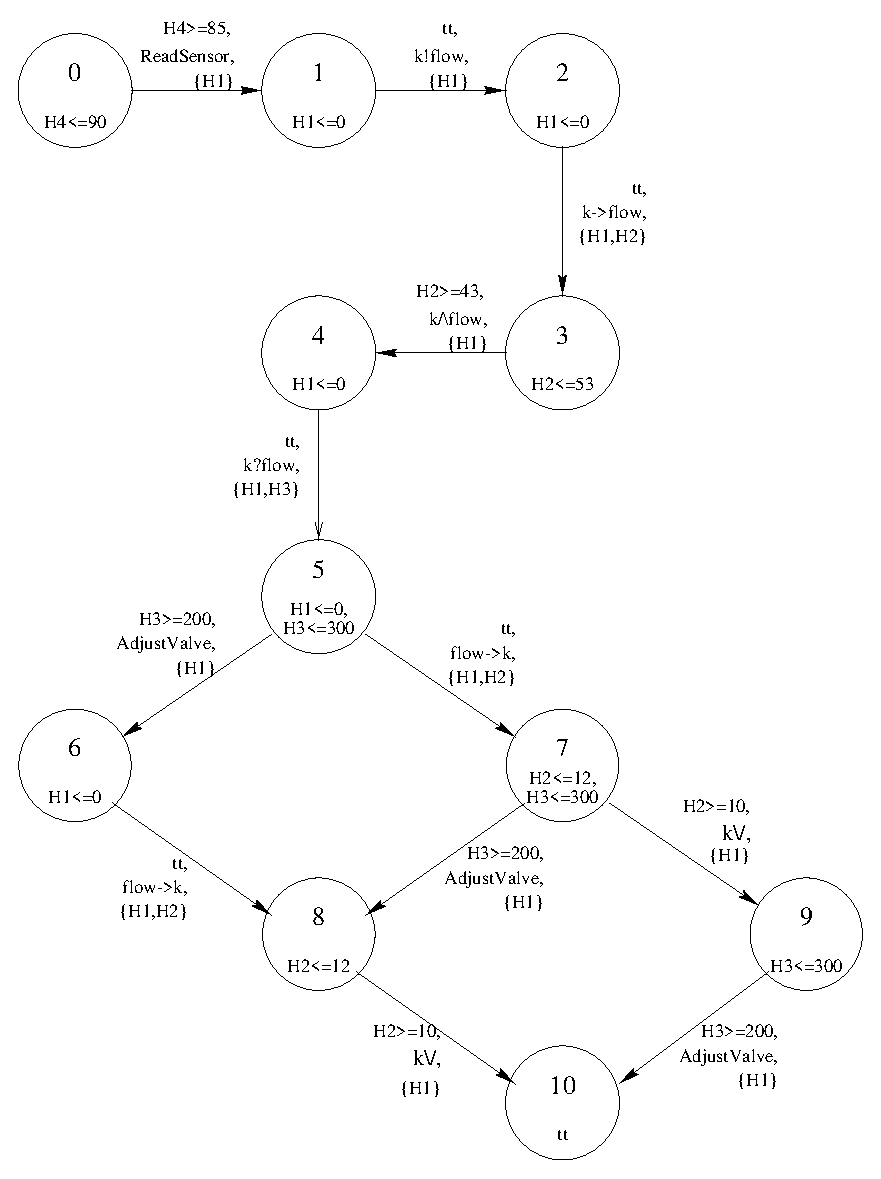
\includegraphics[height=.5\textheight]{TGGEN/tg.eps} %.85\linewidth
\end{center}
\caption{A timed automaton for the one-shot flow regulator\label{fig:tgflowoneshotta}}
\end{figure}  

\section{Models with explicit clocks\label{sec:tgexpclocks}}
Timed automata model the passing of time by using explicit clock
variables.  On the other hand, timed process algebra represent either
absolute or relative time in the syntax of process terms, without the
use of explicit clock variables. This is the case for \bcandle.  As a
first step in the translation from \bcandle\ to timed automata,
explicit clock variables are introduced into \bcandle\ models. The
approach is similar to that adopted in the translation of ATP~\cite{nic:92}.

As an example, look again at the one-shot flow regulator of
Figure~\ref{fig:tgflowoneshot}. Its TA is constructed on the
assumption that the process term has been decorated with clock
variables as follows:
\begin{zed}
[ReadSensor:85,90]^{H4} ; k!flow.x ; \idle \\
| \\ 
k?flow.y ; [AdjustValve:200,300]^{H3} ; \idle
\end{zed}
Similarly, it is assumed that the network channel $\kk$ has been decorated 
with the clock variable $H2$. The clock $H1$ is reserved to enforce 
\emph{urgent} actions, such as $\kk!\ii.\xx$, which must be either executed or
disabled without delay. Now, imagine that time advances by 10 time
units from the initial state, and consider the effect of this time
passage on the term $[ReadSensor:85,90]$. In an unclocked scenario, we
expect to see this term evolve to $[ReadSensor:75,80]$. However, when
using explicit clock variables, we find that $[ReadSensor:85,90]$ remains
unchanged but the value of clock $H4$ advances from $0$ to $10$. In
this case, a $ReadSensor$ transition becomes enabled when the value of
$H4$ reaches 85. Network transitions are controlled similarly by clock
$H2$.

The remainder of this section formalises this idea by 
introducing the basic definitions of explicitly clocked \bcandle\ models.
Throughout, it is assumed that $\clocks$ is the set of clock variables
and $\clock$ ranges over $\clocks$.  

\subsection{Clocked Networks}\label{ss:tgexpclocksnet}
In the case of the network model, each network channel is simply
associated with a clock variable which is used to 
measure the passage of time during message transmission.

Let $\K$ be a finite set of channel identifiers and $\I$ a finite
set of message identifiers. 
\begin{definition}[Clocked Network]
A \emph{clocked network} over $\K$ and $\I$ is a mapping 
$\NN : \K \fun \Channel{\I} \cross \clocks$. The set of clocked networks over
$\K$ and $\I$ is denoted $\NNetwork{\K,\I}$, where 
$\NNetwork{\K,\I} \defs \K \fun \Channel{\I} \cross \clocks$.
\qed
\end{definition}

\begin{remark}\label{rem:tgrestrictnet}
Recall that the constants occurring in 
the clock constraints of the invariant function and edges of a TA
are required to be natural numbers~(\Sec\ref{ss:mscclockconstraints}).
Therefore, it is necessary to restrict attention to clocked networks
in which the transmission latency function of every channel is defined
by a function $\latency : \M \fun \Ninf \cross \Ninf \cross \Ninf
\cross \Ninf$, where $\Ninf \defs \nat \cup \{\infinity\}$ (cf.
Definition~\ref{def:bctransmissionlatency}). We require that all
clocked networks $\NN \in \NNetwork{}$ satisfy this constraint.
\qed
\end{remark}
\begin{notation}
Let $\NN$ be a clocked network and $\NN_\kk = (\channel,\clock)$.
The notation $\channel^\clock$ is used as an abbreviation for
$(\channel,\clock)$. In fact, we sometimes omit the clock variable
entirely when we do not intend to refer to it in some context, and
simply write $\NN_\kk = \channel$.
\end{notation}
\begin{definition}[Clock Variables: Network]
Let $\K$ be a set of channel identifiers.
The clock variables used in a clocked network are given by the
function $\clk : \NNetwork{\K} \fun 2^\clocks$, where 
$\clk(\NN) \defs \{\clock | \kk \in \K \land \NN_\kk = (\_,\clock)\}$
\qed
\end{definition}
\begin{definition}[Unclocked Network]
The \emph{unclocked network} corresponding to a clocked network
is given by the function $\unclk : \NNetwork{\K} \fun \Network{}$, where 
$\unclk(\NN) \defs \{\kk \mapsto \channel | \kk \in \K \land \NN_\kk = 
  (\channel,\_)\}$.
\qed
\end{definition}

\subsection{Clocked Process Terms}\label{ss:tgexpclocksproc}
In defining the set of clocked process terms, we also introduce a
number of syntactic restrictions which ensure that a TA can be
constructed in a straightforward manner:
\begin{enumerate}
\item Constants $\ti_1, \ti_2$ in time-bounded computations 
$[\op:\ti_1,\ti_2]$ are required to be 
natural numbers. This is for similar reasons to those discussed
in Remark~\ref{rem:tgrestrictnet}. 
\item The use of the parallel operator is restricted to the top-level. This
restriction simplifies the implementation of the TA translation.
\item All terms are required to have \emph{static control}. This
is discussed in more detail below.
\end{enumerate}
In practice, these restrictions do not
severely curtail the models which can be expressed.
In fact, we will see that the high-level language \candle\ allows the
expression of a wide variety of systems, and yet all \candle\ programs 
can be translated into \bcandle\ models which satisfy these syntactic
constraints.

The first two restrictions are captured in the following definition of
clocked process terms.
\begin{definition}[Clocked Process Terms]
The set of clocked process terms, $\CProcO{}$, over $\K, \I, \Var, \Op$
and $\G$ is defined inductively by:
\begin{syntax}
\PP & ::= & \QQ \\
    & |   & \PP \parallel \PP \\ \\
\QQ  & ::= &  \kk!\ii.\xx | \kk?\ii.\xx 
            | [\op : t_1, t_2]^\clock | 
            \g \guard \QQ  \\
   & | & \QQ \seqcomp \QQ | \QQ \choice \QQ | \QQ \interrupt \QQ \\
   & | & \rec X.\QQ | X 
\end{syntax}
where $\clocks$ is a set of clocks, $\clock \in \clocks$, $t_1, t_2
\in \Ninf$, $\PP$ ranges over $\CProcO{}$, $\QQ$ ranges over the terms
in $\CProcO{}$ except those containing the parallel operator, and the
other variables are defined as usual (Definition~\ref{def:bcsyntax}).
\qed
\end{definition}
In keeping with our previous convention, we use the variables
$\cbasic, \cbasic', \cbasic_1$ etc. to range over the \emph{clocked basic
terms}, which are of the form $\kk!\ii.\xx$,
$\kk?\ii.\xx$ and $[\op:t_1,t_2]^\clock$.

The definitions over the structure of terms given in
\Sec\ref{sec:bcprocesses} are easily extended to clocked terms, and we shall
refer to \emph{closed} and \emph{guarded} clocked process terms without 
further explanation. The set of closed, guarded, clocked process terms
is denoted $\CProc{}$.

\subsubsection{Static control}
There are some \bcandle\ systems which cannot be represented by any
finite TA. For example, consider a system $(\P,\N,\D) \in \Sys{}$
where the process $\P$ is defined as
\[ \P \defs \rec X.(([a:0] \sq \X) \interrupt ([b:0] \sq \idle)). \]
This can give rise to an unbounded expansion
\[ ((\rec X.[a:0] \sq \X \interrupt [b:0] \sq \idle) \interrupt [b:0] \sq 
\idle) \interrupt \cdots \interrupt [b:0] \sq \idle \]
by repeatedly unwinding the recursion.  In the general case, an
infinite number of locations are required in a TA generated by the
translation of systems containing an unbounded expansion of this sort.
Similar difficulties can be seen with recursion involving parallel and
sequential composition. Clearly, such terms should be excluded from
consideration when proposing a translation scheme to finite TA.

Although, it is difficult to provide a precise characterisation of
the offending terms, it is possible to identify a larger set which
clearly contains all non-finite cases; we call this the set of terms
which \emph{compromise static control}. Roughly speaking, a term
compromises static control if it contains a recursion through the
parallel operator {\tt |} or to the left of the sequential composition
or interrupt operators, {\tt ;} and {\tt [>}. This idea is stated formally
in the following definition:
\begin{definition}[Static control]
A term $\P \in \Proc{}$ \emph{compromises static
control} if $\P$ is of the form $\rec X.\P_1$ and any of the following
conditions hold:
\begin{enumerate}
\item $\P_1$ contains a sub-term of the form $\Q | \R$ and 
  $X \in \fv(\Q) \cup \fv(\R)$;
\item $\P_1$ contains a sub-term of the form $\Q \sq \R$ and 
  $X \in \fv(\Q)$;
\item $\P_1$ contains a sub-term of the form $\Q \interrupt \R$
  and $X \in \fv(\Q)$. 
\end{enumerate}
A term $\P \in \Proc{}$ \emph{has static control} iff $\P$ does not
contain any term which compromises static control.  A \bcandle\ system
$(\P,\N,\D) \in \Sys{}$ \emph{has static control} iff $\P$ has static
control.
\qed
\end{definition}
This definition is extended naturally to clocked process terms.
However, notice that by restricting the use of the parallel operator
to the top-level in clocked terms, there is no possibility of static
control being compromised by a clocked term satisfying condition (1).
The benefits of restricting attention to systems having static control
can be summarised as follows~\cite{gar:92}:
\begin{itemize}
\item A finite TA can be constructed for systems with static control. 
\item The property of static control is decidable using a simple and
  efficient algorithm.
\item It is easy for the system developer to understand the constraint
  and to develop models which satisfy it.
\item TA construction for systems with static control
  can be implemented efficiently.
\item Most systems of practical interest can be modelled within the 
  required constraint.
\end{itemize}
Unless stated otherwise, we assume from now on that clocked process terms 
have static control.

\subsubsection{Operations on clocked process terms}
There are a number of operations on the syntax of clocked terms which are
useful. The functions $\clk$, $\iclk$ and $\unclk$ are defined below.
\begin{definition}[Clock Variables]
The clock variables of a clocked process term 
are identified by the function $\clk : \CProcO{} \fun 2^\clocks$,
defined as the least set satisfying:
\begin{eqnarray*}
\clk([\op:t_1,t_2]^\clock) & = & \{\clock\} \\
\clk(\kk!\ii.\xx) & = & \clk(\kk?\ii.\xx)  = \clk(X) = \emptyset \\
\clk(\g \guard \PP_1) & = & \clk(\PP_1) \\
\clk(\PP_1 \genop \PP_2) & = & \clk(\PP_1) \cup \clk(\PP_2), \quad \genop\; \in
\{\sq,\choice,\interrupt,\parallel\} \\
\clk(\rec X.\PP_1) & = & \clk(\PP_1)
\end{eqnarray*}
\qed
\end{definition}
\begin{definition}[Initial Clock Variables]\label{def:tgiclk}
The \emph{initial} clock variables of a clocked process term, $\PP$, 
are identified by the function $\iclk : \CProcO{} \fun 2^\clocks$,
defined as the least set satisfying:
\begin{eqnarray*}
\iclk([\op:t_1,t_2]^\clock) & = & \{\clock\} \\
\iclk(\kk!\ii.\xx) & = & \iclk(\kk?\ii.\xx)  = \emptyset \\
\iclk(\g \guard \PP_1) & = & \emptyset \\
\iclk(\PP_1 \sq \PP_2) & = & \iclk(\PP_1) \\
\iclk(\PP_1 \genop \PP_2) & = & \iclk(\PP_1) \cup \iclk(\PP_2), \quad \genop\; \in
\{\choice,\interrupt,\parallel\} \\
\iclk(\rec X.\PP_1) & = & \iclk(\PP_1[\rec X.\PP_1/X])
\end{eqnarray*}
where $\iclk(\PP)$ is well defined iff $\PP$ is guarded.
\qed
\end{definition}
\begin{definition}[Unclocked process term]\label{def:tgunclk}
The unclocked process term corresponding to a clocked process term
is given by the function $\unclk : \CProcO{} \fun \ProcO{}$, where 
$\unclk(\PP)$ is defined by:
\begin{eqnarray*}
\unclk(\kk!\ii.\xx) & \defs & \kk!\ii.\xx \\ 
\unclk(\kk?\ii.\xx) & \defs & \kk?\ii.\xx \\
\unclk([\op:\ti_1,\ti_2]^\clock) & \defs & [\op:\ti_1,\ti_2] \\
\unclk(\g\guard\PP_1) & \defs & \g\guard\unclk(\PP_1) \\
\unclk(\PP_1\genop\PP_2) & \defs & \unclk(\PP_1) \genop \unclk(\PP_2), \quad\genop\; \in \{\sq,\choice,\interrupt,\parallel\} \\
\unclk(\rec X.\PP_1) & \defs & \rec X.\unclk(\PP_1) \\
\unclk(X) & \defs & X 
\end{eqnarray*}
\qed
\end{definition}
These operations are illustrated in the following small example.
\begin{exampleb}
Let $\PP$ be the clocked process term defined by
\begin{zed}
\PP \defs \rec X . ([Init:t_1]^{H1} \sq \kk?flow.\xx \sq 
                    [TestFlow:t_2]^{H2} \sq \\ 
\t2                (FlowOk \guard [Delay:t_3]^{H3} \choice
                    FlowHigh \guard \kk!alarm.\xx \sq \idle)) \sq X
\end{zed}
Then, $\clk(\PP)$ gives the set of all clock variables used in $\PP$,
i.e.  $\clk(\PP) = \{H1,H2,H3\}$. The set $\iclk(\PP) = \{H1\}$ gives
the set of clocks which can influence the initial behaviour of
$\PP$. Finally, the unclocked term $\unclk(\PP)$ is just $\PP$ with all clock
variables removed:
\begin{zed}
\unclk(\PP) = \rec X . ([Init:t_1]\sq\kk?flow.\xx \sq [TestFlow:t_2] \sq \\
\t2                 (FlowOk \guard [Delay:t_3] \choice
                    FlowHigh \guard \kk!alarm.\xx \sq \idle)) \sq X
\end{zed}
\qed
\end{exampleb}

\subsection{Safe Clock Allocations}
So far, we have imposed no constraints on how clocks can be allocated
to process terms and networks. Efficiency suggests that we should use
as few clock variables as possible. However, it is clear that some clock
allocations will cause problems. For example, consider the clocked term
\begin{zed}
\hspace*{-1cm}
[ReadSensor:10]^{H1} \sq [LogData:20]^{H1} \sq \idle 
|  
[ComputeSetPoint:15]^{H1} \sq \idle\;.
\end{zed}
The $ReadSensor$ transition should reset $H1$ so that it can be used
to measure the progress of $LogData$. On the other hand, if
$ReadSensor$ resets $H1$, then the passage of time for the
$ComputeSetPoint$ computation will not be measured properly: the reset
of $H1$ at time 10 will delay the execution of $ComputeSetPoint$ until
time 25, which is clearly not the intended behaviour. Similar
difficulties can be observed with clock allocations to network
channels. The problem exists when two or more system components share
the use of a clock variable but do not agree on the instants when it
should be reset.  In this case, we say that the system exhibits
\emph{clock (variable) contention}, otherwise it is said to be
\emph{contention free}.

In the absence of recursion, we can be sure that a system can never
evolve to one which exhibits clock contention if the sets of clock
variables allocated to process terms involved in an interrupt or
parallel composition are disjoint, and each network channel also has
its own distinct clock variable. However, with recursion, even this
restriction is not enough to remove the possibility of clock contention.
\begin{exampleb}
Consider the term 
\[ \PP \defs \rec X . [a:2]^{H1} \sq ([b:1]^{H1} \sq [c:2]^{H1} 
                                        \interrupt X).
\] 
Ignoring network and data environment, we see that $\PP$ can evolve
by the passage of two units of time, and the execution of an $a$-action,
to the term
\[ [b:1]^{H1} \sq [c:2]^{H1} \interrupt 
      (\rec X . [a:2]^{H1} \sq ([b:1]^{H1} \sq [c:2]^{H1} 
                                        \interrupt X)).
\]
Now, when the $b$-action is executed after the passage of one 
further time unit, we see the problem of clock variable contention. On the
one hand, clock $H1$ should be reset in order to begin timing the
computation $[c:2]^{H1}$, but, on the other hand, $H1$ must not be
reset since it is currently required in timing the computation
$[a:2]^{H1}$.
\qed
\end{exampleb}
This example prompts us to introduce one final restriction on the
syntax of process terms, namely, that in any term of the form
$\PP_1 \interrupt \PP_2$, the term $\PP_2$ must be guarded.

\noindent
These ideas are summarised by the notion of a \emph{safely clocked process 
term}. 
\begin{definition}[Safely clocked process term]
$\PP \in \CProc{}$ is said to be \emph{safely clocked} iff
all sub-terms $\PP'$ of $\PP$ satisfy 
\begin{enumerate}
\item if $\PP'$ is of the form $\PP_1 \interrupt \PP_2$, then
$\PP_2$ is guarded, and the initial clock 
variables of $\PP_2$ do not occur in the clock variables of $\PP_1$, i.e
$\clk(\PP_1) \cap \iclk(\PP_2) = \emptyset$, and
\item if $\PP'$ is of the form $\PP_1 \parallel \PP_2$, then the clock 
variables of $\PP_1$ and $\PP_2$ are disjoint, i.e. 
$\clk(\PP_1) \cap \clk(\PP_2) = \emptyset$. 
\qed
\end{enumerate}
\end{definition}
Clearly, if $\PP$ is a safely clocked process term, then $\PP$ is
contention free. 

\noindent
For the sake of completeness, the formal definition of a \emph{safely clocked
network} is given as follows.
\begin{definition}[Safely clocked network]
A clocked network $\NN \in \NNetwork{\K}$ is said to be \emph{safely
clocked} if each channel is associated with a distinct clock
variable, i.e. if \\
\hspace*{2cm} 
$\forall \kk,\kk' \in \K | \kk \neq \kk' 
  \such \NN_\kk = (\_,\clock) \land \NN_{\kk'} = (\_,\clock') \implies \clock 
    \neq \clock'$. 
\qed
\end{definition}

It can be shown that the edge relation of a TA constructed by the
method of~\Sec\ref{sec:tgcons} preserves the safety of clock
allocation, i.e. if a location $\tgloc$ is safely clocked and there
are $\clkcond_1,\ldots,\clkcond_n$, $\any_1,\ldots,\any_n$ and
$\resets_1,\ldots,\resets_n$ ($n \geq 0$) such that $\tgloc = \tgloc_0
\goes{\clkcond_1,\any_1,\resets_1}
\tgloc_1 \cdots \goes{\clkcond_n,\any_n,\resets_n} \tgloc_n = \tgloc'$, then
$\tgloc'$ is safely clocked. The property of static control is
essential for the proof, which is a long but straightforward induction
and is omitted. An obvious corollary is that if the initial location
is safely clocked, then all reachable locations are contention free.

The requirement of safe clock allocation is stronger than strictly necessary
to ensure that the sort of problems mentioned above are avoided. However,
it is a simple property which can be checked statically, and will be enforced 
throughout, unless its relaxation is explicitly stated and justified.

\subsection{Clocked \bcandle\ systems}
The definitions are extended to \bcandle\ systems in an obvious way.
\begin{definition}[Clocked \bcandle\ systems] 
The set $\CSys{}$ of clocked \bcandle\ systems is the set of triples
$(\PP,\NN,\D)$ where $\PP \in \CProc{}$ is a safely clocked process term with
static control, $\NN$ is a safely clocked network in $\NNetwork{}$, 
$\D$ is a data environment in $\DataEnv{}$, and the following conditions are 
satisfied:
\begin{itemize}
\item the sets of process and network clocks are disjoint, i.e.
$\clk(\PP) \cap \clk(\NN) = \emptyset$;
\item the corresponding unclocked system $(\unclk(\PP),\unclk(\NN),\D)$ 
is a \bcandle\ system in $\Sys{}$.
\qed
\end{itemize}
\end{definition}
\begin{definition}[Clock Variables: \bcandle\ system]
The clock variables of a \bcandle\ system $\csys \in \CSys{}$
are identified by the function $\clk : \CSys{} \fun 2^\clocks$,
where $\clk(\PP,\NN,\D) \defs \clk(\PP) \cup \clk(\NN)$.
\qed
\end{definition}
\begin{definition}[Unclocked \bcandle\ system]
The unclocked \bcandle\ system corresponding to a clocked
\bcandle\ system is given by the function $\unclk : \CSys{} \fun \Sys{}$,
where $\unclk(\PP,\NN,\D) \defs (\unclk(\PP),\unclk(\NN),\D)$.
\qed
\end{definition}

\section{Timed Automaton Construction\label{sec:tgcons}} 
\subsection{Principles of construction}
The TA for a clocked \bcandle\ system $\csys \in \CSys{}$ has some subset
of $\CSys{}$ as its set of locations with $\csys$ as the initial location.
The set $\clocks$ of clocks comprises the set $\clk(\csys)$ of clocks
occurring in $\csys$, together with a distinct \emph{urgent} clock
$\uclock \notin \clk(\csys)$, used in enforcing immediate actions.
The set $\Actions$ of actions contains the sets of process and network
actions $\ProgLabels \cup \NetLabels$. The definition of the
construction of the edges of the TA closely follows the standard
semantic rules for the corresponding unclocked system
(\Sec\ref{sec:bcformalmodel}). For each rule in the semantics which
justifies a transition labelled with a discrete action, there is a
corresponding rule which introduces an edge in the
automaton. Similarly, the rules which justify the time transitions are
captured by the definition of the invariant function~$\tginv$. This
style of presentation, adopted also in~\cite{nic:92,db:96}, emphasises
the relationship between the semantics of a system model and its
associated TA.
 
\subsection{Construction of the automaton}\label{ss:tgmktgraph}
We begin by explaining the notion of \emph{structurally reachable} location 
which is a useful auxiliary concept in the definition of the TA construction.
 
A location $\tgloc$ is structurally reachable if there is a sequence
of edges from the initial location $\tgiloc$ to $\tgloc$, i.e.
there are $\clkcond_1,\ldots,\clkcond_n$, $\any_1,\ldots,\any_n$ and
$\resets_1,\ldots,\resets_n$ ($n \geq 0$) such that
$\tgiloc = \tgloc_0 \goes{\clkcond_1,\any_1,\resets_1} \tgloc_1 \cdots
\goes{\clkcond_n,\any_n,\resets_n} \tgloc_n = \tgloc$. The structurally
reachable part of an automaton $\AA$ is the automaton $\sreach(\AA)$
which is given by the restriction to structurally reachable
locations. We use the term ``structural reachability'' for this
concept since it is based on the structure of an automaton as a directed
graph, and is different from the usual concept of reachability in the
transition system of the automaton (see Definitions~\ref{def:mscreach}
and~\ref{def:msctgsem}).
\begin{definition}
Let $\AA = (\tglocs,\tgiloc,\Actions,\tgclks,\tgedges,\tginv)$ be an
automaton.  Then, the structurally reachable part of $\AA$ is denoted
$\sreach(\AA)$ and is defined to be the automaton
$(\tglocs',\tgiloc,\Actions,\tgclks,\tgedges',\tginv')$, where
\begin{itemize}
\item $\tglocs'$ is the least set satisfying
\begin{enumerate}
\item $\tgiloc \in \tglocs'$
\item if $\tgloc \in \tglocs'$ and $(\tgloc,\_,\_,\_,\tgloc') \in
\tgedges$ then $\tgloc' \in \tglocs'$
\end{enumerate}
and
\item $\tgedges' = \tgedges \cap (\tglocs' \cross \ClockConstraints \cross 
  \Actions \cross 2^\clocks \cross \tglocs')$
\item $\tginv' = \tginv \cap (\tglocs' \cross \ClockConstraints)$
\qed
\end{itemize}
\end{definition}

\begin{remark}\label{rem:tgsreacheq}
For any TA $\AA$, it is clear that the transition systems
of $\AA$ and $\sreach(\AA)$ are strongly equivalent.
\end{remark}

Now, we can formally define the construction of a TA corresponding to a
\bcandle\ system.
\begin{definition}[Timed automaton construction]\label{def:tgconstruct}
The timed automaton for a clocked \bcandle\ system $\csys \in
\CSys{}$ is denoted $\Gr(\csys)$, where 
$\Gr(\csys) \defs \sreach(\GrPlus(\csys))$ and $\GrPlus(\csys)$ is the
automaton $(\tglocs,\tgiloc,\Actions,\tgclks,\tgedges,\tginv)$, where
\begin{itemize}
\item $\tglocs = \CSys{}$ is the set of locations.
\item $\tgiloc = \csys$ is the initial location. 
\item $\Actions = \ProgLabels \cup \NetLabels$ is the set of 
  action labels.
\item $\tgclks = \clk(\csys) \cup \{\uclock\}$ is the set of clock variables,
  where $\uclock \notin \clk(\csys)$.
\item $\tgedges$ is the least set of edges which is closed under the rules 
  of figures~\ref{fig:netedges}, \ref{fig:basicedges}, \ref{fig:seqchedges} 
  and~\ref{fig:intparedges}.
  The rules make use of generic labels $\prog, \netw$ and
  $\any$, where $\prog$ ranges over $\ProgLabels$, $\netw$ ranges over 
  $\NetLabels$ and $\any$ ranges over $\Actions$.
\item $\tginv : \tglocs \fun \ClockConstraints$ is the invariant function
  as defined in Definition~\ref{def:tginvariant}.  
\qed
\end{itemize}
\end{definition}

\begin{definition}[Invariant Function]\label{def:tginvariant}
Let $\clocks$ be a set of clock variables and
let $\csys \in \CSys{}$ be a clocked \bcandle\ system, where $\clk(\csys)
\cup \{\uclock\} \subseteq \clocks$.
The \emph{invariant function}, $\tginv : \CSys{} \fun \ClockConstraints$ 
is as defined in Figure~\ref{fig:tginvariant}.
\qed
\end{definition}

\begin{figure*}
\begin{minipage}{\linewidth}
\small
\setlength{\extrarowheight}{5ex}
\begin{center}
\begin{tabular}{|ll|}
\hline 
\multicolumn{2}{|c|}{\gpre} \\
\multicolumn{2}{|c|}{\gaccpt} \\
\multicolumn{2}{|c|}{\gpost} \\
\multicolumn{2}{|c|}{\gfree} \\
\hline
\end{tabular}
\end{center}
\end{minipage}
\caption{Rules for Network Edges\label{fig:netedges}}
\end{figure*}

\begin{figure*}
\begin{minipage}{\linewidth}
\small
\setlength{\extrarowheight}{5ex}
\begin{center}
\begin{tabular}{|ll|}
\hline 
\multicolumn{2}{|c|}{\gsnda} \\
\multicolumn{2}{|c|}{\gsndb} \\
\multicolumn{2}{|c|}{\grcva} \\
\multicolumn{2}{|c|}{\grcvb} \\
\multicolumn{2}{|c|}{\gcompa} \\
\multicolumn{2}{|c|}{\gcompb} \\
\hline
\end{tabular}
\end{center}
\end{minipage}
\caption{Rules for Basic System Edges\label{fig:basicedges}}
\end{figure*}

\begin{figure*}
\begin{minipage}{\linewidth}
\small
\setlength{\extrarowheight}{5ex}
\begin{center}
\begin{tabular}{|ll|}
\hline 
\multicolumn{2}{|c|}{\ggua} \\
\multicolumn{2}{|c|}{\ggub} \\
\multicolumn{2}{|c|}{\gseqa} \\
\multicolumn{2}{|c|}{\gseqb} \\
\multicolumn{2}{|c|}{\gcha} \\
\multicolumn{2}{|c|}{\gchb} \\
\multicolumn{2}{|c|}{\gchc} \\
\multicolumn{2}{|c|}{\grec} \\
\hline
\end{tabular}
\end{center}
\end{minipage}
\caption{Rules for Guard, Sequential Composition, Choice and Recursion Edges\label{fig:seqchedges}}
\end{figure*}

\begin{figure*}
\begin{minipage}{\linewidth}
\small
\setlength{\extrarowheight}{5ex}
\begin{center}
\begin{tabular}{|ll|}
\hline 
\multicolumn{2}{|c|}{\ginta} \\
\multicolumn{2}{|c|}{\gintb} \\
\multicolumn{2}{|c|}{\gintc} \\
\multicolumn{2}{|c|}{\gintd} \\
\multicolumn{2}{|c|}{\gpara} \\
\multicolumn{2}{|c|}{\gparb} \\
\multicolumn{2}{|c|}{\gparc} \\
\multicolumn{2}{|c|}{\gpard} \\
\multicolumn{2}{|c|}{\gpare} \\
\hline
\end{tabular}
\end{center}
\end{minipage}
\caption{Rules for Interrupt and Parallel Composition Edges\label{fig:intparedges}}
\end{figure*}

\begin{figure*}
\begin{eqnarray*}
\tginv(\PP,\NN,\D) & \defs & \tginv(\PP,\D) \land \tginv(\NN) \\
\tginv(\kk!\ii.\xx,\D) & \defs & \uclock \leq 0 \\
\tginv(\kk?\ii.\xx,\D) & \defs & \cctrue \\
\tginv([\op:t_1,t_2]^\clock,\D) & \defs & \ite{t_2 \in \nat}{\clock \leq t_2}{\cctrue} \\
\tginv(\g \guard \PP,\D) & \defs & \ite{\D \models \g}{\uclock \leq 0}{\cctrue} \\
\tginv(\PP_1 \sq \PP_2,\D) & \defs & \tginv(\PP_1,\D) \\
\tginv(\PP_1 \genop \PP_2,\D) & \defs & \tginv(\PP_1,\D) \land \tginv(\PP_2,\D) \quad \genop\; \in
\{\choice,\interrupt,\parallel\} \\
\tginv(\rec X.\PP,\D) & \defs & \tginv(\PP[\rec X.\PP/X],\D) \\
\tginv(\NN) & \defs & \bigwedge_{\kk \in \K} \tginv(\NN_\kk) \\
\tginv(\free,\emptyseq)^\clock & \defs & \cctrue \\
\tginv(\free,\mm:\mq)^\clock & \defs & \uclock \leq 0 \\
\tginv(\preact{t_1,t_2}{\mm},\mq)^\clock & \defs & \ite{t_2 \in \nat}{\clock \leq t_2}{\cctrue} \\
\tginv(\offers{\mm},\mq)^\clock & \defs & \uclock \leq 0 \\
\tginv(\postact{t_1,t_2}{\mm},\mq)^\clock & \defs & \ite{t_2 \in \nat}{\clock \leq t_2}{\cctrue} 
\end{eqnarray*}
\caption{Invariant function $\tginv : \CSys{} \fun \ClockConstraints$ \label{fig:tginvariant}}
\end{figure*}

\subsection{Commentary on the construction}\label{ss:tgcomments}
The translation of a \bcandle\ system to its associated TA is
straightforward for the most part. However, there are some aspects
which require clarification. These concern the treatment of data and
the enforcement of urgent transitions. These points are considered below.

\subsubsection{Treatment of Data}
The TA constructed by the method described here are exactly the timed
safety automata (TSA) defined in~\cite{hnsy:94}. These automata have
been studied extensively and can be analysed automatically using tools
such as \break KRONOS~\cite{bdm:98}. The choice of TSA as the target of the
translation from \bcandle\ directs the translation process in a number
of ways.  In the treatment of data, it requires that each distinct
reachable data environment gives rise to at least one distinct
location in the corresponding TA. Very often, this leads to the
creation of a TA with a large number of locations. Other approaches
which accommodate explicit data in TA models have avoided this problem
by working with extended automata; the usual extension being to allow
the use of conditions over data variables on edges, in addition to
conditions over clock variables, see for
example~\cite{tri:98,her:98,bll:98,blt:99}. A single location may then
represent many control states, each having a different data
environment.  If the user is expected to create a system model
explicitly as a network of TA, then the handling of data is done most
sensibly using extended automata of this sort. Certainly, one would
not wish to construct by hand the automata which are created by our
method.  However the situation is not so clear when creating automata
automatically from some other input language, as is the case here for
\bcandle. For although the construction may give rise to many more
locations in the TA than a construction for extended automata, it does
not lead to an increase in the number of states in the simulation
graph (\Sec\ref{sec:mscsimgraph}), which is the primary structure over
which most analyses are performed and whose size is their main
constraining factor.  This point will be considered further in
Chapter~\ref{chap:sggen}.
 
\subsubsection{Urgent transitions}
There are several operations in \bcandle\ which must either be executed 
or disabled \emph{without delay}, such operations are called \emph{urgent}.
The urgent operations of the process component of a \bcandle\ model are
\begin{itemize}
\item all send operations, $\kk!\ii.\xx$, 
\item data guarded operations, $\g \guard \P$, when the guard $\g$ is 
  satisfied, and 
\item computations for which the upper bound is 0, i.e.
  computations of the form $[\op:0,0]$.
\end{itemize}
The urgent network operations are
\begin{itemize}
\item the commencement of the transmission of the highest priority pending 
  message when a channel is free and its message queue is not empty, i.e.
  transitions of the form $\kk\preact{}{\mm}$, and
\item the commencement of the post-acceptance phase of message transmission,
  i.e. transitions of the form $\postact{}{\mm}\kk$.
\end{itemize}
The urgency of these operations is enforced in a TA by using a single distinct 
clock variable $\uclock$, which is reset on every edge and which is used
in the invariant $\uclock \leq 0$, attached to all
locations in which an urgent transition is enabled. Notice that the
clock guard on all urgent transitions is $\cctrue$.

\begin{proposition}\label{prop:tgresetuclock}
Let $\csys \in \CSys{}$ be a clocked \bcandle\ system and
$\Gr(\csys) = (\tglocs, \tgiloc, \Actions, \clocks, \tgedges, \tginv)$
the TA constructed from $\csys$ according to Definition~\ref{def:tgconstruct}.
Then, for any edge $\tgedge = (\tgloc,\clkcond,\any,\resets,\tgloc') \in 
\tgedges$, the urgent clock is reset by $\tgedge$, i.e. $\uclock \in \resets$. 
\end{proposition}
\begin{proof}
Induction on the depth of the inference justifying the existence of the 
edge. Intuitively, one can see that $\uclock$ is reset by every
basic process and network edge and that the resets are propagated by all
process operators.
\end{proof}

\subsection{Correctness of the construction}\label{ss:tgcorrect}
The TA generated from a \bcandle\ system model yields a transition system
which is strongly equivalent to that given by the standard \bcandle\ semantics.
Therefore, we can be confident that conclusions reached by analysing the
TA are valid for the system model. We state 
the equivalence formally below but relegate the details of the proof to 
Appendix~\ref{app:proofs}.
\begin{proposition}\label{prop:tgcorrect}
Let $\csys \in \CSys{}$ be a clocked \bcandle\ system and
$\sys \defs \unclk(\csys)$ the corresponding unclocked system.
Let $\Gr(\csys)$ be the TA given by 
Definition~\ref{def:tgconstruct}. Then, the transition systems
of $\Gr(\csys)$ and $\sys$ are strongly equivalent.
\[
\TSys{\Gr(\csys)} \bisim \TSys{\sys}
\]
\end{proposition}
\begin{proof}
Appendix~\ref{app:proofs}.
\end{proof}

\section{Implementation of the construction \label{sec:tggraphimpl}}
Although \Sec\ref{ss:tgmktgraph} gives a precise description of the TA
which corresponds to a \bcandle\ system, it does not give a practical
method for constructing it. 

A significant difficulty, in practice, concerns the size of the
representation of locations $(\PP,\NN,\D) \in \CSys{}$. In particular,
the representation of the control component $\PP$ by an algebraic term
results in implementations which are extremely inefficient in their
use of computer memory. Moreover, a construction of the TA based upon
repeated construction and/or comparison of the TA of the sub-systems,
is not time-efficient.

Similar problems have been observed by Garavel in the translation of
LOTOS~\cite{gar:92}, and by Yovine in the translation of
ATP~\cite{yov:93}. We adapt their solutions to our system models, in
developing an approach which accommodates both explicit data values
and dense real-time.  In this approach, the translation of a system
model into a TA is performed in two stages:
\begin{itemize}
\item in the first stage, a compact, intermediate form, similar to a Petri 
net~\cite{mur:89}, is constructed for the system model;
\item in the second stage, the TA itself is constructed efficiently 
using the net built in the first stage.
\end{itemize}
The main advantage of using a net as an intermediate representation is
that it is then possible to represent the control component of a system
state by a marking of the net. This representation is likely to be
much more compact than the abstract syntax tree of the corresponding
process term, and it leads to algorithms with a reduced need to
manipulate sub-terms.

The remainder of this section is concerned with the development of an
efficient method for constructing the TA of a \bcandle\ system $\csys$, i.e.  
with the construction of $\Gr(\csys)$.

\subsection{Nets} \label{ss:tgnets}
\subsubsection{Introduction}
The nets which are used in this work are not strictly Petri nets but
are close to the extended nets of~\cite{yov:93}. As usual, a net
consists of a set of \emph{places} and a set of \emph{transitions}; the
convention used here is to denote a set of places by $\W,\W',\W_1$
etc. and a set of transitions by $\T,\T',\T_1$ etc. Two main
extensions are introduced.
\begin{enumerate}
\item Each transition has an associated \emph{attribute} which is used 
in determining whether or not the transition is \emph{fireable} in a
given system \emph{context}, where a context consists of a network and
a data environment. This is in accord with many of the varieties of
generalised or interpreted Petri net~\cite{kel:76,sif:77}.
\item In addition to a source set of places which must be \emph{marked} 
in order for a transition to be fireable, and a target set of places
to which control flows when a transition fires, each transition is
also associated with a set of places which are said to be
\emph{vulnerable} to the firing of the transition. When a transition
fires, control is removed not only from the places in its source set
but also from all those places which are vulnerable to it. This
extension allows a compact representation of the interrupt operator in
particular.
\end{enumerate} 

\begin{exampleb}
Figure~\ref{fig:examplenet} shows an example net. 
\begin{figure}[h]
\begin{center}
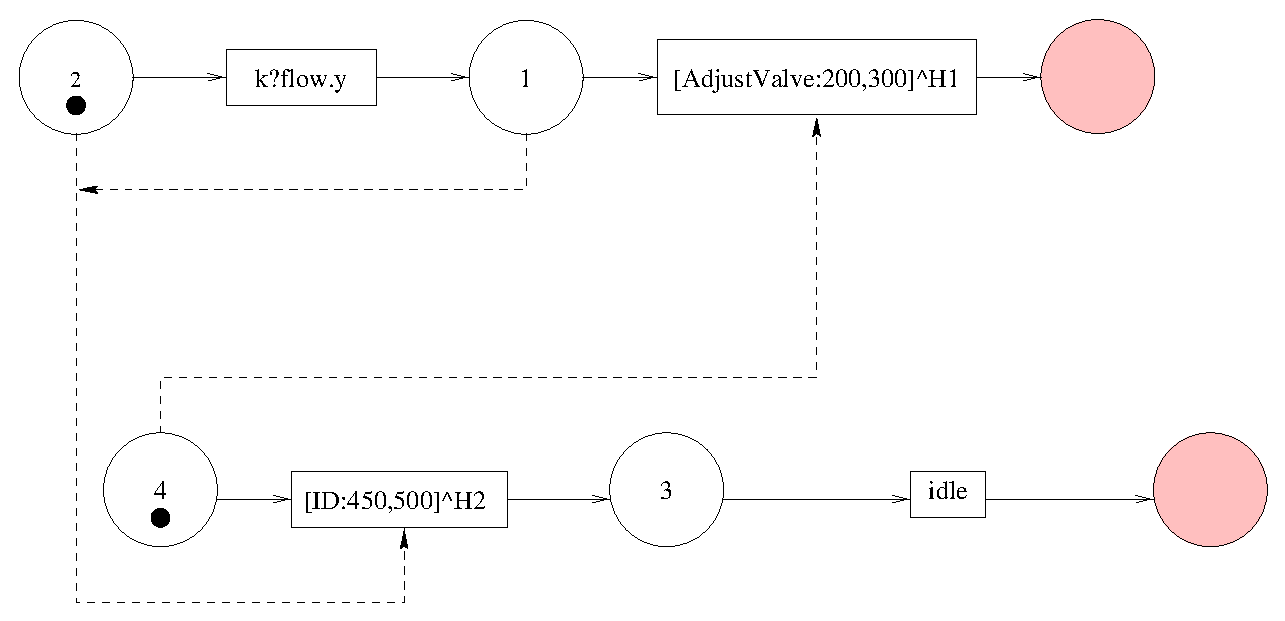
\includegraphics[width=.8\linewidth]{TGGEN/interrupt.eps}
\end{center}
\caption{Example Net\label{fig:examplenet}}
\end{figure}
It represents the process term $\kk?flow.y \sq
[AdjustValve:200,300]^{H1} \interrupt [450,500]^{H2} \sq \idle$. The
places of the net are shown as circles and the transitions as
boxes. The shaded circles represent a distinguished place
$\tickpl$\footnote{In the diagram of a net, we often have more than
one shaded circle, in order to simplify the layout. All such shaded
circles should be interpreted as representing the same $\tickpl$
place.}, modelling termination. A label inside a transition box
denotes the transition attribute, e.g., $\kk?flow.y$.  The standard
flow relation is shown using solid lines, e.g., if place 2 is marked,
and the context allows, the transition $\kk?flow.y$ can fire, removing
a token from place 2 and adding a token to place 1.  The vulnerability
relation is shown using dashed lines, e.g., places 1 and 2 are
vulnerable to the firing of the transition $[ID:450,500]^{H2}$, so a
token in either of those places is removed when the transition fires.
The small black circles in places 2 and 4 show that those places are
marked.
\qed
\end{exampleb}
Nets are introduced formally below.

\subsubsection{Definitions and Notation}
Let $\CProc{}$ be a set of clocked process terms over process variables
$\XX$, predicate names $\G$ and clocks $\clocks$. The set $\TAttrib$
of \emph{transition attributes} is defined:
\begin{syntax}
\tattrib & ::= & \cbasic | \gu{\g} | X
\end{syntax}
where $\tattrib \in \TAttrib$ is a transition attribute, $\cbasic \in
\CProc{}$ is a clocked basic term and $X \in \XX$ is a process
variable. We use the notation $\gu{\g}$ to denote a transition
attribute consisting of the predicate name $\g \in \G$.

The set of clocks associated with a transition attribute $\tattrib$ is
denoted $\clk(\tattrib)$, where 
$\clk([\op:t_1,t_2]^\clock) \defs  \{\clock\}$, and $\clk(\tattrib) \defs
\emptyset$, for any attribute $\tattrib$ of the form $\kk!\ii.\xx$, 
$\kk?\ii.\xx$, $\gu{\g}$, and $X$. 

A net can now be defined as follows.
\begin{definition}[Net]
A net is a tuple $\RR = (\W,\T,\WI)$ where
\begin{itemize}
\item $\W$ is the set of \emph{places}
\item $\T \subseteq \W \cross 2^\W \cross \TAttrib \cross 2^\WTick$ is the set
  of \emph{transitions}. $\WTick$ denotes the set of places $\W
  \cup \{\tickpl\}$ in which $\tickpl \notin \W$ is a distinguished
  place used in the representation of the terminal process $\tick$.
\item $\WI \subseteq \W$ is the set of \emph{initial} places 
\qed
\end{itemize}
\end{definition}
Let $\RR = (\W,\T,\WI)$ be a net and $\tr = (\ww,\WV,\tattrib,\WT) \in \T$
a transition. We adopt the following conventions:
\begin{itemize}
\item $\ww \in \W$ is the \emph{trigger} of $\tr$, denoted $\preset{\tr}$.
\item $\WV \subseteq \W$ is the set of places \emph{vulnerable to} $\tr$,
  denoted $\vset{\tr}$
\item $\tattrib \in \TAttrib$ is the \emph{attribute} of $\tr$, denoted $\attr{\tr}$
\item $\WT \subseteq \W$ is the \emph{target} set of $\tr$, denoted 
  $\postset{\tr}$   
\end{itemize}  

In the case that a place $\ww$ is the trigger of exactly one
transition, the transition triggered by $\ww$ is
denoted by $\tr_\ww$. Every place in a net constructed from a
\bcandle\ system according to the method of \Sec\ref{sec:consnet} is the
trigger of exactly one transition.

A \emph{marking} is a set of places. The marking $\WI$ is the
\emph{initial marking}. Let $\W$ be a marking. For each transition
$\tr$, if $\preset{\tr} \in \W$, then $\tr$ is said to be
\emph{conditionally enabled} in $\W$.
  
Let $\RR_i = (\W_i,\T_i,\WI_i)$ for $i \in \{1,2\}$, be two nets. $\RR_1$ and
$\RR_2$ are said to be \emph{disjoint} iff 
$\W_1 \cap \W_2 = \emptyset$.
 
The set of clocks associated with a set $\W$ of places is denoted
$\clk(\W)$, where $\clk(\W) \defs \bigcup_{\ww \in \W}
\clk(\tattrib\tr_\ww)$. 

\subsubsection{Behaviour}
The semantics of a net is given with respect to a system context which
comprises a network and a data environment. The semantics is given as
a transition system between states consisting of a marking of the net
and a context.  Given a net $\RR = (\W,\T,\WI)$, a state $(\PP,\NN,\D)
\in \CSys{}$ can be represented by $(\W_1,\NN,\D)$ where $\W_1 \subseteq
\W$ is a marking of $\RR$ which represents the control component
$\PP$. Intuitively, a system can evolve from one state
$(\W_1,\NN,\D)$ to another state $(\W_2,\NN',\D')$ as the result of
either a process transition or a network transition.

For a process transition, assume $\ww \in \W_1$ and that $\ww$ is the
trigger of some transition $\tr$.  If the context $\NN, \D$ satisfies
the conditions required by the attribute $\tattrib\tr$, then a new marking
$\W_2$ is created from $\W_1$ by removing $\ww$ and any places which
are vulnerable to $\tr$, and then including all of the target places 
of $\tr$. The new context, $\NN', \D'$ is created according to the
requirements of the attribute $\tattrib\tr$. 

In the case of a network transition, the system may evolve to a
new state, in which the network component is modified, but the
marking and data environment remain unchanged. However, notice that
a network transition is inhibited by a marking as follows:
\begin{itemize}
\item  a message offer cannot be removed if some process is ready to accept it,
i.e., a network transition to the post-acceptance phase of transmission
of a message with identifier $\ii$ on a channel $\kk$ is not allowed
if the current marking contains a place which is the trigger of a
transition whose attribute is $\kk?\ii.\xx$ for some data variable
$\xx$.
\end{itemize}
These ideas are presented formally in the rules {\bfseries R.1} and
{\bfseries R.2} below.
\begin{definition} \label{def:tgnetrules}
Let $\RR = (\W, \T, \WI)$ be a net, $\W_1 \subseteq \W$. Let $\NN$ be
a clocked network over sets $\K$ of channel identifiers and $\I$ of
message identifiers.  Let $\D$ be a data environment.

The process transitions of $(\W_1,\NN,\D)$ are given
by the rule:
\begin{center}
\rfirea  \label{def:Rone}
\end{center}

and the network transitions by the rule:
\begin{center}
\rfireb \label{def:Rtwo}
\end{center}
where 
\begin{itemize}
\item
the $\fire$ relation, as given in Figure~\ref{fig:fire}, simply recasts
the semantic rules for basic terms and guards, in defining the behaviour of
each transition attribute in a given system context, and 
\item 
$\awaited(\W,\kk,\ii)$ holds iff, in the marking $\W$, it is possible to 
receive from channel $\kk$ a message with identifier $\ii$. Formally, \\
\hspace*{2cm} $\awaited(\W,\kk,\ii) \defs \{\ww \in \W | \attr{\tr_\ww} = \kk?\ii.\_\} \neq \emptyset$
\qed
\end{itemize}
\end{definition}


\begin{figure*}
\begin{minipage}{\linewidth}
\small
\setlength{\extrarowheight}{5ex}
\begin{center}
\begin{tabular}{|ll|}
\hline 
\multicolumn{2}{|c|}{\fsnda} \\
\multicolumn{2}{|c|}{\frcva} \\
\multicolumn{2}{|c|}{\fcompa} \\
\multicolumn{2}{|c|}{\fgua} \\
\hline
\end{tabular}
\end{center}
\end{minipage}
\caption{Rules for $\fire$\label{fig:fire}}
\end{figure*}

\subsection{Constructing the net for a clocked term} \label{sec:consnet}
Let $(\PP,\NN,\D) \in \CSys{}$ be a \bcandle\
system. In this section, it is shown how to construct the net for
$\PP$, denoted $\mknet{\PP}$.  We begin by considering the
construction of nets for the basic terms.  The construction of a net
for a compound term, $\PP_1 \sq \PP_2$, $\PP_1 \choice \PP_2$, $\PP_1
\interrupt \PP_2$ and $\PP_1 \parallel \PP_2$, proceeds compositionally 
from the nets for $\PP_1$ and $\PP_2$.


\subsubsection{Basic Terms}
The net for each of the clocked basic terms, $\cbasic \in \CProc{}$ is
constructed in the same way for each. A new place is
created to act as the trigger of a transition whose attribute is the
term itself and whose outgoing arc leads to the distinguished place,
$\tickpl$.

\begin{exampleb}
Let $\cbasic$ be the term
$\kk?flow.\yy$. Figure~\ref{fig:basicnet} shows the net given by
$\mknet{\cbasic}$. 
\begin{figure}[h]
\begin{center}
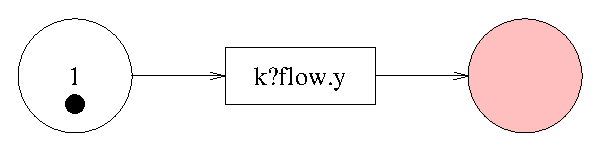
\includegraphics[width=.4\linewidth]{TGGEN/basic.eps}
\end{center}
\caption{Net for a basic term\label{fig:basicnet}}
\end{figure}
The figure shows the initial marking of the
net. The terminal place $\tickpl$ is shown as a shaded circle. Place
(1) is the trigger of the net's only transition, whose attribute is
shown inside the box, and whose target set is the singleton
$\{\tickpl\}$.
\qed
\end{exampleb}

\begin{definition}
Let $\cbasic$ be one of the basic terms $\kk!\ii.\xx$,
$\kk?\ii.\xx$ or $[\op:t_1,t_2]^\clock$. Then the net for $\cbasic$, is
constructed as follows:
\[\mknet{\cbasic} \defs (\{\ww\},\{(\ww,\{\},\cbasic,\{\tickpl\})\},\{\ww\}) \]
where $\ww \neq \tickpl$ is a place.
\qed
\end{definition}

\subsubsection{Sequential Composition}
In constructing the net of the sequential composition, $\PP_1 \sq
\PP_2$, all that needs to be done is to combine the nets of $\PP_1$ and 
$\PP_2$ and then modify each transition $\tr$ of $\PP_1$, which leads
to the immediate termination of $\PP_1$, so that it leads instead to
the initial places of $\PP_2$. This represents the transfer of control
from a termination point in $\PP_1$ to the starting point(s) of
$\PP_2$.  A transition $\tr$ leads to immediate termination iff its
target set, $\postset{\tr}$, is $\{\tickpl\}$. The transfer of control
is implemented simply by making $\postset{\tr}$ equal to the initial
places of $\PP_2$.
\begin{exampleb}
Consider the term $\kk?flow.y \sq [AdjustValve:200,300]^{{H1}}$.  Its
net is constructed very simply, as shown in Figure~\ref{fig:seqnet}.
\qed
\end{exampleb}
\begin{figure}[h]
\begin{center}
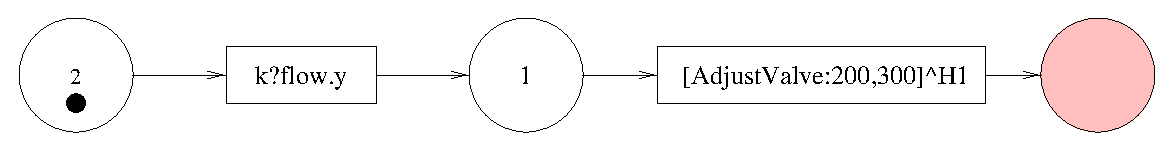
\includegraphics[width=.8\linewidth]{TGGEN/seq.eps}
\end{center}
\caption{Net for a sequential composition\label{fig:seqnet}}
\end{figure}   
\begin{definition}
Let $(\W_i,\T_i,\WI_i) = \mknet{\PP_i}, \text{ for } i \in \{1,2\}$, be 
disjoint nets. The net $\mknet{\PP_1 \sq \PP_2}$ for the sequential
composition $\PP_1 \sq \PP_2$ is given by
\[\mknet{\PP_1 \sq \PP_2} \defs (\W_1 \cup \W_2, \T'_1 \cup \T_2,\WI_1)\] where
\begin{eqnarray}
\T'_1 & \defs & \{\tr | \tr \in \T_1 \land \postset{\tr} \neq \{\tickpl\}\} \nonumber
\\[.3mm]
& \cup & \{ (\preset{\tr},\vset{\tr},\attr{\tr},\WI_2) | \tr \in \T_1
\land \postset{\tr} = \{\tickpl\}\} \nonumber 
\end{eqnarray}
\qed
\end{definition}

\subsubsection{Guard}
A guarded process $\g \guard \PP$ evaluates the guard $\g$ in its
current data environment and then behaves as $\PP$ if the guard is true or
simply idles otherwise. We construct a net rather as if $\g$ is a basic
term and $\guard$ is sequential composition.
\begin{exampleb}
Let $\PP$ be the term $Shutdown \guard \idle$. Figure~\ref{fig:guardnet}
shows the net given by $\mknet{\PP}$.
\qed
\end{exampleb}
\begin{figure}[h]
\begin{center}
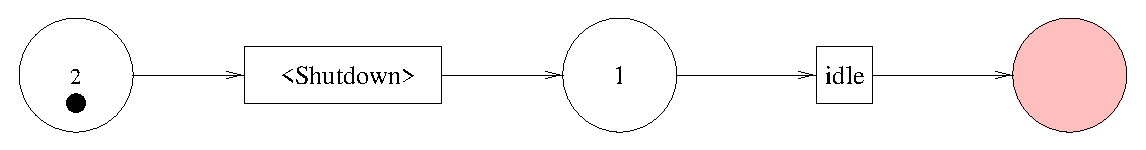
\includegraphics[width=.8\linewidth]{TGGEN/guard.eps}
\end{center}
\caption{Net for a data-guarded term\label{fig:guardnet}}
\end{figure}
\begin{definition}
Let $\mknet{\PP} = (\W,\T,\WI)$, then the net of $\g \guard \PP$ is
given by
\[\mknet{\g \guard \PP} \defs (\W \cup \{\ww\},\T \cup
\{(\ww,\{\},\gu{\g},\WI)\},\{\ww\}) \]
where $\ww \notin \WTick$ is a place.
\qed
\end{definition}
  
\subsubsection{Choice}
A choice, $\PP_1 \choice \PP_2$, is resolved in favour of the process
which is first able to perform an initial transition,
the possibility of action then being removed from the other
process. The removal of control is represented in the net for $\PP_1
\choice \PP_2$ by adjusting the vulnerable sets of the transitions of
each process, so that control is removed from one process whenever an
action occurs in the other.
\begin{exampleb} \label{xmpl:choice} \mbox{\strut} \break
Let $\PP_1 = \kk?flow.y \sq [AdjustValve:200,300]^{H1}$ and $\PP_2 =
[450,500]^{H2} \sq \idle$. The term $\PP_1 \choice \PP_2$ models the
situation in which one of two possible behaviours can occur: either a
\emph{flow} message is received on channel $\kk$ within 500 time
units and then the process adjusts a valve; or a \emph{flow}
message is not received for at least 450 time units, after which the
timeout may elapse and the process idles
forever. Figure~\ref{fig:choicenet} shows the net which is constructed
for $\mknet{\PP_1 \choice \PP_2}$.  
\begin{figure}[h]
\begin{center}
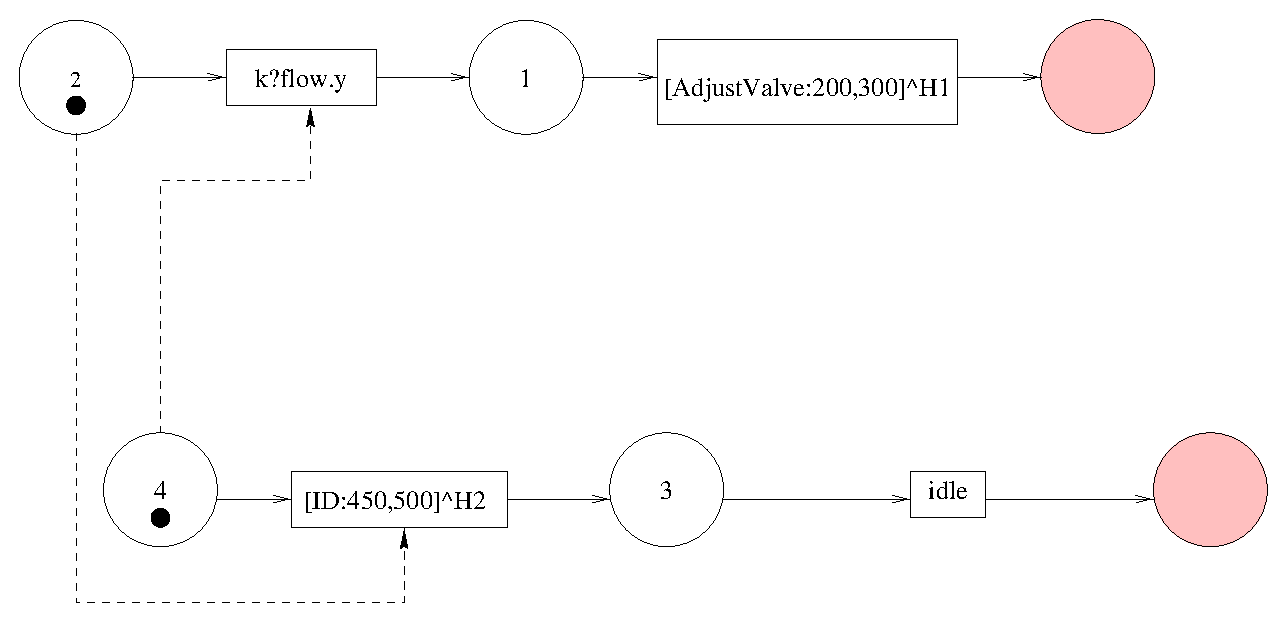
\includegraphics[width=.8\linewidth]{TGGEN/choice.eps}
\end{center}
\caption{Net for a choice\label{fig:choicenet}}
\end{figure}
Notice that the marking of the net
shows the initial possibility of both behaviours. The places which are
\emph{vulnerable to} a transition are indicated with a dashed line,
directed from each vulnerable place to the transition(s) to which it
is vulnerable. For example, place 4 is vulnerable to the transition
$k?flow.y$. This means that if $k?flow.y$ fires, then
a token residing at place 4 will be removed, and so the transition which
is triggered by it will be disabled. 
\qed
\end{exampleb}
\begin{definition}  
Let $(\W_i,\T_i,\WI_i) = \mknet{\PP_i}, \text{ for } i \in \{1,2\}$, 
be disjoint nets. Then
\[\mknet{\PP_1 \choice \PP_2} \defs (\W_1 \cup \W_2, \T, \WI_1 \cup \WI_2)\] where
\begin{eqnarray*}
\T & \defs & \{\tr | \tr \in \T_1 \land \preset{\tr} \notin \WI_1\} \\
   & \cup  & \{(\preset{\tr},\vset{\tr} \cup \WI_2,\attr{\tr},\postset{\tr}) |
                 \tr \in \T_1 \land \preset{\tr} \in \WI_1\} \\
   & \cup  & \{\tr | \tr \in \T_2 \land \preset{\tr} \notin \WI_2\} \\
   & \cup  & \{(\preset{\tr},\vset{\tr} \cup \WI_1,\attr{\tr},\postset{\tr}) |
                 \tr \in \T_2 \land \preset{\tr} \in \WI_2\} \quad\quad\quad\quad\qed
\end{eqnarray*}
\end{definition}

\subsubsection{Interrupt}
An interrupt, $\PP_1 \interrupt \PP_2$, differs from choice in that
control is only removed from $\PP_2$ when a \emph{terminating}
transition of $\PP_1$ occurs. So $\PP_1$ can perform transitions
while $\PP_2$ retains the possibility of action. Wherever control
resides in $\PP_1$, it is removed upon the occurrence of an initial 
transition of $\PP_2$. 
\begin{exampleb}\mbox{\strut}\break
Let $\PP_1 = \kk?flow.y \sq [AdjustValve:200,300]^{H1}$ and $\PP_2 =
[450,500]^{H2} \sq \idle$. The term $\PP_1 \interrupt \PP_2$ behaves similarly
to $\PP_1 \choice \PP_2$ which was considered in Example~\ref{xmpl:choice};
the primary difference being that $[450,500]^{H2}$ acts as a watchdog timer
rather than a timeout: i.e., it remains active throughout the behaviour
of $\PP_1$ and is only disabled when $\PP_1$ terminates. This difference 
is reflected in the construction of the net for $\PP_1 \interrupt \PP_2$
shown in Figure~\ref{fig:interruptnet}. 
\begin{figure}[h]
\begin{center}
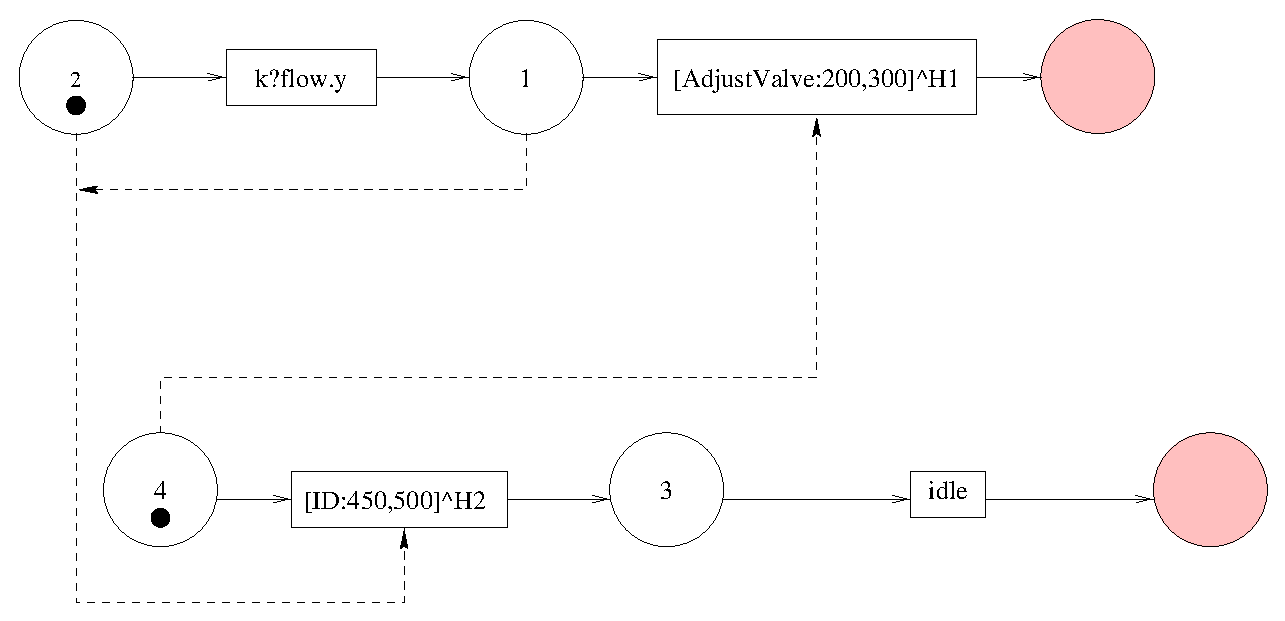
\includegraphics[width=.8\linewidth]{TGGEN/interrupt.eps}
\end{center}
\caption{Net for an interrupt\label{fig:interruptnet}}
\end{figure}
Attention should be given to the following points:
\begin{itemize}
\item the triggers of \emph{all} transitions associated with $\PP_1$
  are made vulnerable to the initial transition of $\PP_2$, and  
\item the trigger of the initial transition of $\PP_2$ is vulnerable only
  to the \emph{terminating} transition of $\PP_1$. 
\end{itemize}
The effect of this is that $[ID:450,500]^{H2}$ remains fireable even
after $k?flow.y$ has fired, and, if $[ID:450,500]^{H2}$ is fired, then
both $k?flow.y$ \emph{and} $[AdjustValve:200,300]^{H1}$ are disabled.
Contrast this with the net for choice in Figure~\ref{fig:choicenet}.
\qed
\end{exampleb}
\begin{definition}
Let $(\W_i,\T_i,\WI_i) = \mknet{\PP_i}, \text{ for } i \in \{1,2\}$, be
disjoint nets. Then
\[\mknet{\PP_1 \interrupt \PP_2} \defs (\W_1 \cup \W_2, \T, \WI_1 \cup \WI_2)\] where
\begin{eqnarray*}
\T & \defs & \{\tr | \tr \in \T_1 \land \postset{\tr} \neq \{\tickpl\}\} \\
   & \cup  & \{(\preset{\tr},\vset{\tr} \cup \WI_2,\attr{\tr},\postset{\tr}) |
                   \tr \in \T_1 \land \postset{\tr} = \{\tickpl\}\} \\
   & \cup  & \{\tr | \tr \in \T_2 \land \preset{\tr} \notin \WI_2\} \\
   & \cup  & \{(\preset{\tr},\vset{\tr} \cup \W_1,\attr{\tr},\postset{\tr}) |
                 \tr \in \T_2 \land \preset{\tr} \in \WI_2\} 
\end{eqnarray*}
\qed
\end{definition}

\subsubsection{Parallel Composition}
Control in a parallel composition, $\PP_1 \parallel \PP_2$, is maintained
independently in each process. Moreover, the parallel operator occurs
only at the top-level, i.e. we never encounter terms such as 
$(\PP_1 \parallel \PP_2) \sq \PP_3$. In this case, the net for 
$\PP_1 \parallel \PP_2$ can be constructed simply as the independent nets 
for $\PP_1$ and $\PP_2$.
\begin{definition}
Let $(\W_i,\T_i,\WI_i) = \mknet{\PP_i}, \text{ for } i \in \{1,2\}$, be
disjoint nets. Then
\[\mknet{\PP_1 \parallel \PP_2} \defs (\W_1 \cup \W_2, \T_1 \cup \T_2, \WI_1 \cup \WI_2)\]
\qed
\end{definition}
The benefits of the restricted use of parallelism can be seen here in
the very simple net translation and in the fact that it is possible to
support the translation of \bcandle\ into nets in which every
transition requires only a single trigger. The use of such simple nets 
has consequent benefits in the efficiency of the implementation of the
TA construction which is based on them.

\subsubsection{Process Variable}
A process variable, $X$, represents a recursion point. As such, it has
a net representation consisting of a place which is the trigger of a
single transition whose target set is empty initially and 
is finalised later in the construction, on encountering the binding,
$\rec X$. There is sure to be such a binding since we are dealing only
with closed terms.  Notice also that because of the restriction to systems
with static control, a free process variable cannot be encountered on the left
of a sequential composition and so the target set of the net for the process
variable remains unchanged until the binding is encountered.
\begin{definition}
Let $X$ be a process variable. The net of $X$ is defined:
\[\mknet{X} \defs (\{\ww\},\{(\ww,\{\},X,\{\})\},\{\ww\}) \]
where $\ww \neq \tickpl$ is a place.
\qed
\end{definition}

\subsubsection{Recursion Operator}
The construction of the net for the recursion operator, $\rec X.\PP$,
involves the resolution of the target sets of all those transitions in the
net for $\PP$ whose attribute is the free process variable $X$. 
If $(\W,\T,\WI)$ is the net constructed for $\PP$, then each
such target set is made equal to the set, $\WI$, of initial places of
$\PP$; i.e., the `knot is tied'.
\begin{exampleb}
Consider the term 
\[\rec Flow.[ReadSensor:85,90]^{H1} \sq \kk!flow.\xx \sq Flow\] which models control in a system
which repeatedly reads a flow sensor, storing the reading in the
variable $x$, and transmits its value on channel $\kk$. Its net is
shown in Figure~\ref{fig:recursionnet}; 
\begin{figure}[h]
\begin{center}
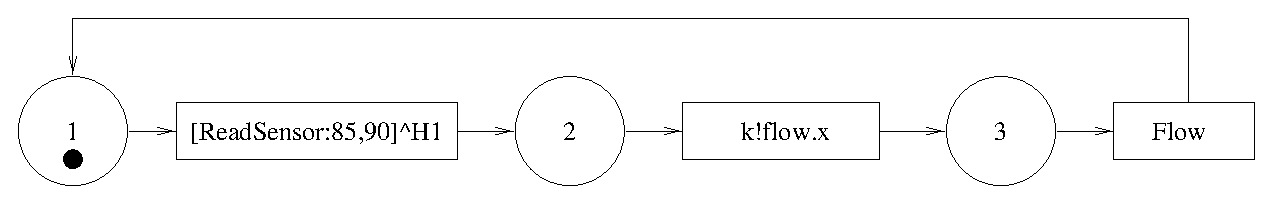
\includegraphics[width=.8\linewidth]{TGGEN/rec1.eps}
\end{center}
\caption{Net for a recursion\label{fig:recursionnet}}
\end{figure}
the knot is tied simply in
this case by returning control to the beginning of the process.
Notice that control is returned \emph{indirectly} from
$\kk!flow.\xx$ to the start of the process at place 1 via the
transition $Flow$ triggered by place 3. A more compact net can
be used in which the redundant place and transition (place 3 and $Flow$) 
are omitted and in which control is returned directly from
$\kk!flow.\xx$ to the beginning of the process (see
Figure~\ref{fig:recursionneta}). 
\begin{figure}[h]
\begin{center}
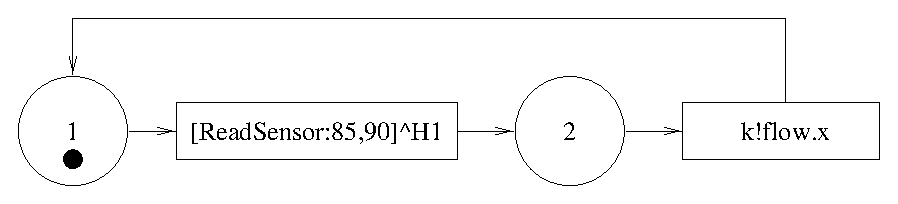
\includegraphics[width=.65\linewidth]{TGGEN/rec2.eps}
\end{center}
\caption{Compact net for a recursion\label{fig:recursionneta}}
\end{figure}
It will be shown later how such indirections can be systematically
removed and we will assume that this is always done in the nets which
we construct.
\qed
\end{exampleb}
\begin{definition}
Let $\mknet{\PP} = (\W,\T,\WI)$, then the net of $\rec X.\PP$ is given by
\[ \mknet{\rec X.\PP} \defs (\W,\T',\WI) \] where
\begin{eqnarray}
\T' & \defs & \{\tr | \tr \in \T \land \attr{\tr} \neq X\} \nonumber \\[.3mm]
  & \cup & \{(\preset{\tr},\vset{\tr},\attr{\tr},\WI) | \tr \in \T
                   \land \attr{\tr} = X\} \nonumber
\end{eqnarray}
\qed
\end{definition}

\subsubsection{Removing indirections}\label{ss:removeind}
The net of a recursive process, constructed using the approach
described above, contains places and transitions whose only purpose is
to redirect the flow of control via a recursion point.  Such
transitions, which we have called \emph{indirections}, have a process
variable for their attribute. We can remove each of these transitions
from the net, and also the places which trigger them, and transfer
control directly to the start of the process. This avoids the
generation of redundant locations and edges in the construction of the
TA of the process. An algorithm is presented shortly which gives a
method for the removal of indirections. First, we give an example which
has been constructed to illustrate its most significant features.
\begin{exampleb}
Consider the term
\[ \PP \defs \rec X.[a:1]^{H1} \sq (X \choice stop \guard [b:0]^{H1} \sq \idle)\]
which models a process which repeatedly executes an $a$ action until
the predicate $stop$ becomes $\True$ when it executes a single $b$
action and then idles forever. The net for this process, including
indirections, is shown in Figure~\ref{fig:indirection}.   
\begin{figure}[h]
\begin{center}
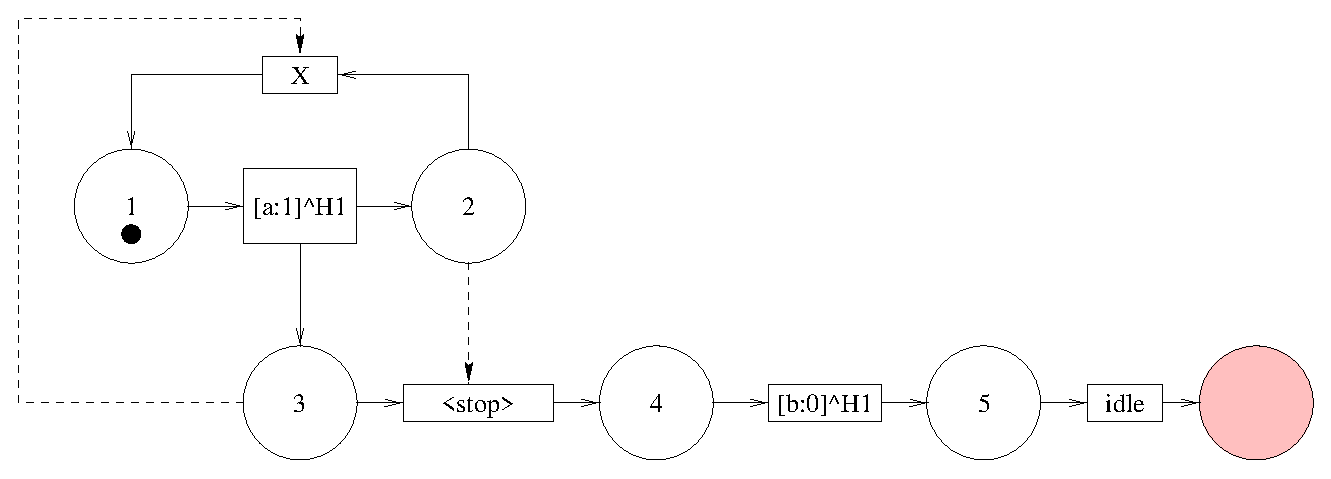
\includegraphics[width=.8\linewidth]{TGGEN/ind1.eps}
\end{center}
\caption{A recursion with indirections\label{fig:indirection}}
\end{figure}
For the most part, the net is unremarkable. But, notice that the
unguarded process variable $X$, in the term $(X \choice stop \guard
[b:0]^{H1} \sq \idle)$, does not cause problems in the net
representation: the term $\PP$ is represented by the net as shown, and
the term $\PP \choice stop \guard [b:0]^{H1} \sq \idle$, which is
reached after the recursion is unwound, is represented by the same net
with the marking $\{1,3\}$.  The net contains a single indirection,
namely the transition whose attribute is $X$ and whose trigger is the
place labelled 2. The result of removing this indirection is shown in
Figure~\ref{fig:indirectionremoved}.
\begin{figure}[h]
\begin{center}
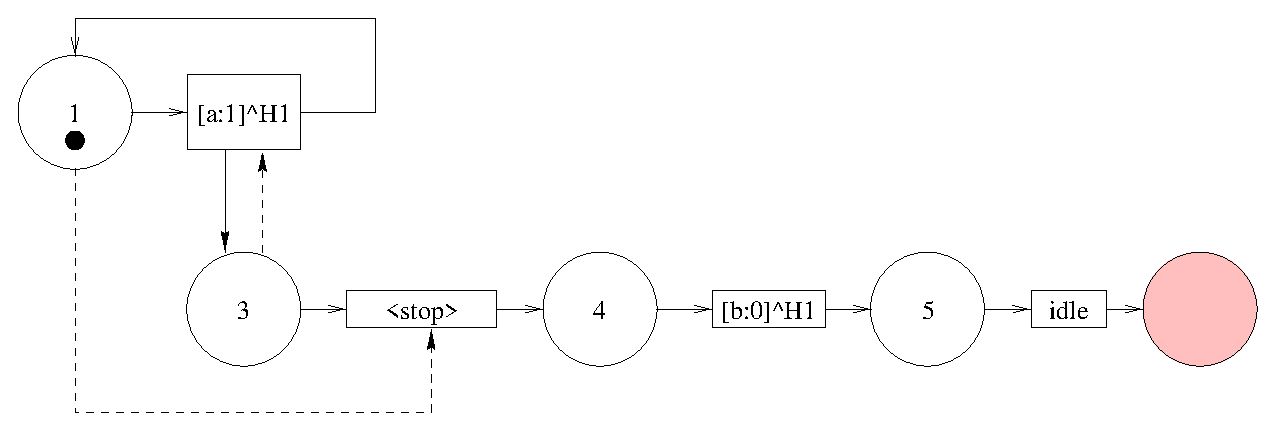
\includegraphics[width=.8\linewidth]{TGGEN/ind2.eps}
\end{center}
\caption{A recursion with indirections removed\label{fig:indirectionremoved}}
\end{figure}
In order
to remove the indirection we need to perform the following steps:
\begin{enumerate}
\item Modify those transitions which are directed towards
the indirection -- in this case there is just one such transition,
$[a:1]^{H1}$ -- so that they bypass the indirection and are directed 
to its target set instead -- in this case, the place labelled 1.
\item Modify vulnerable sets to take account of the above change. There are
two cases in which vulnerable sets need to be altered:
\begin{enumerate}
\item If an indirection is vulnerable to some transition $\tr$ then all 
places to which it directs control should become vulnerable to $\tr$. In
Figure~\ref{fig:indirection}, 2 is vulnerable to $\gu{stop}$, 
so in the modified net (Figure~\ref{fig:indirectionremoved}) 1 has become 
vulnerable to this transition.
\item Any places which are vulnerable to the indirection should instead
be made vulnerable to those transitions to which control is directed
by it. Notice in Figure~\ref{fig:indirection} that 3 is vulnerable to
$X$, whereas in the modified net of
Figure~\ref{fig:indirectionremoved}, this place is vulnerable instead
to $[a:1]^{H1}$.
\qed 
\end{enumerate} 
\end{enumerate}
\end{exampleb}
The algorithm in Figure~\ref{fig:removeindirections} formalises a method
for the removal of indirections. 
\begin{figure}
\begin{center}
\small
\NumberProgramstrue
\begin{programbox}
\INPUT
\text{A net } (\W,\T,\WI) \text{ constructed as described in~\Sec\ref{sec:consnet}}  
\ENDINPUT
\OUTPUT
\text{A new, equivalent net, } (\W',\T',\WI) \text{, which does not contain indirections.}
\ENDOUTPUT
\BEGIN
\I := \set{\tr | \attr{\tr} = X, \text{for any process variable X}}
\W' := \W \setminus \set{\preset{i} | i \in \I}
\T' := \T \setminus \I 
\FOREACH \tr \in \T' \DO
\FOREACH i \in \I \DO
\IF \preset{i} \in \postset{\tr} \THEN \postset{\tr} := \postset{\tr} \setminus \{\preset{i}\} \cup \postset{i} \FI
\IF \preset{i} \in \vset{\tr} \THEN \vset{\tr} := \vset{\tr} \setminus \{\preset{i}\} \cup \postset{i} \FI
\IF \preset{\tr} \in \postset{i} \THEN \vset{\tr} := \vset{\tr} \cup \vset{i} \FI 
\OD
\OD
\END
\end{programbox}
\end{center}
\caption{Algorithm to remove indirections \label{fig:removeindirections}}
\end{figure}
The following remarks are intended to explain this algorithm.
$\I$ is the set of indirections, $\T'$ is the set of all
transitions \emph{except} indirections, $\W'$ is the set of all places
\emph{except} those which are the trigger of some indirection.  For
each transition $\tr \in \T'$ and for each indirection $i \in \I$, the
algorithm first causes the indirection to be bypassed (line~11); then
all those places to which the indirection directs control
are made vulnerable to $\tr$, if $i$ is vulnerable to $\tr$~(line~12); finally,
if $i$ directs control to $\tr$ then all places vulnerable to $i$ are
made vulnerable to $\tr$ (line~13).

\subsection{Final stage of timed automaton construction}
The final stage of the construction of the TA for a system
$(\PP,\NN,\D)$ is to build the automaton itself, based on the net
$\mknet{\PP}$ constructed in the previous stage. 
If $\RR = (\W,\T,\WI)$ is the net for $\PP$, then a simple and efficient 
algorithm can be used to generate the TA for $(\PP,\NN,\D)$ by
starting from the initial location $(\WI,\NN,\D)$ and visiting
all reachable locations under the relation $\goesr{}$ as defined by
rules \textbf{R.1} and \textbf{R.2} (Definition~\ref{def:tgnetrules}).
A standard reachability algorithm is employed for this
purpose (Figure~\ref{fig:tgmkgraph}). The following definition gives the 
details.
\begin{definition} \label{def:tgconstructautomaton} 
Let $(\PP,\NN,\D) \in \CSys{}$ be a clocked \bcandle\ system. 
Let $\RR = (\W,\T,\WI)$ be the net $\mknet{\PP}$. Then, the TA 
$\GrImpl(\PP,\NN,\D) \defs
(\tglocs,\tgiloc,\Actions,\tgclks,\tgedges,\tginv)$ is built as follows:
\begin{itemize}
\item The set $\tglocs$ of locations is as given when the algorithm in 
Figure~\ref{fig:tgmkgraph} terminates.
\item The initial location $\tgiloc$ is $(\WI,\NN,\D)$.
\item The set $\Actions$ of action labels is 
$\ProgLabels \cup \NetLabels$.
\item The set $\tgclks$ of clocks is the set of clocks associated with
the attributes of the transitions in $\T$, together with the network clocks
and the urgent clock $\uclock$,
i.e., $\tgclks \defs \clk(\W) \cup \clk(\NN) \cup \{\uclock\}$, where
$\uclock \notin \clk(\W) \cup \clk(\NN)$.
\item The set $\tgedges$ of edges is as given when the algorithm in 
Figure~\ref{fig:tgmkgraph} terminates.
\item The invariant function $\tginv : \tglocs \fun \ClockConstraints$ is 
given by
\begin{eqnarray*}
\tginv(\W,\NN,\D) & \defs & \tginv(\W,\D) \land \tginv(\NN) \\
\tginv(\W,\D) & \defs & \bigwedge_{\ww \in \W} \tginv(\attr\tr_\ww, \D) \\
\end{eqnarray*}
where $\tginv(\cbasic,\D)$ and $\tginv(\NN)$ are as in Definition~\ref{def:tginvariant} and 
\[ \tginv(\gu{\g},\D) \defs  \ite{\D \models \g}{\uclock \leq 0}{\cctrue} \]
\qed
\end{itemize} 
\end{definition}

\begin{figure}
\NumberProgramstrue
\begin{center}
\small
\begin{programbox}
\INPUT
  \text{A \bcandle\ system } (\PP,\NN,\D) 
  \text{A net } \RR = (\W,\T,\WI) = \mknet{\PP}
\ENDINPUT
\OUTPUT
  \text{The set of locations } \tglocs
  \text{The set of edges } \tgedges
\ENDOUTPUT
\BEGIN
\tglocs := \{(\WI,\NN,\D)\}
WAITING := \{(\WI,\NN,\D)\}
\tgedges := \emptyset
\WHILE WAITING \neq \emptyset \DO
  \text{remove some } \tgloc \text{ from } WAITING
  \tgedges' := \{(\tgloc,\tgguard,\any,\resets,\tgloc') \vbar \tgloc  \goesr{\tgguard,\any,\resets} \tgloc'\}
  \tgedges := \tgedges \cup \tgedges' 
  \FOREACH (\_,\_,\_,\_,\tgloc') \in \tgedges' \DO
    \IF \tgloc' \notin \tglocs
      \text{add } \tgloc' \text{ to } \tglocs
      \text{add } \tgloc' \text{ to } WAITING
    \FI
  \OD
\OD
\END
\end{programbox}
\end{center}
\caption{Algorithm to construct a timed automaton\label{fig:tgmkgraph}}
\end{figure}
For any clocked \bcandle\ system $\csys \in \CSys{}$, we conjecture that
$\GrImpl(\csys)$ is isomorphic to $\Gr(\csys)$, and so, from
Proposition~\ref{prop:tgcorrect}, we
conclude that its transition system is strongly equivalent to the
corresponding \bcandle\ system $\unclk(\csys)$. The proof of the conjecture
is left to future work.

\section{A simple example}\label{sec:tgexample}
In order to illustrate the automatic TA construction method, we return
to the example of the simple flow regulator~(\Sec\ref{sec:bcexample}).
For ease of reference, the \bcandle\ model is presented again in
Figure~\ref{fig:tgflowagain}. We briefly describe the various stages
of the translation of the model to a TA.
\begin{figure}
\small
\begin{verbatim}
      Flow | Valve

      where

      Flow = [ReadSensor:85,90] ; k!flow.x ; idle 
                 [> [PERIOD:10000,10250] ; Flow

      Valve = k?flow.y ; [AdjustValve:200,300]; Valve

      network
      /*          pri dlb dub dlB duB   */
        k = (flow : 1, 43, 53, 10, 12)

      data x, y
\end{verbatim}
\caption{The flow regulator revisited\label{fig:tgflowagain}}
\end{figure}

Initially, the source file containing the model description is parsed,
and equational definitions are rewritten as recursive process
terms. Next, the clock variables are allocated. This gives the
following clocked process term:
\begin{zed}
((\rec Flow.(([ReadSensor:85,90]^{H3} ; (k!flow.x ; \idle)) \\
\t1 \interrupt ([PERIOD:10000,10250]^{H5} ; Flow))) \\
| \\ 
(\rec Valve.(k?flow.y ; ([AdjustValve:200,300]^{H4} ; Valve))))
\end{zed}
The static components of each network channel are constructed from the
details given in the network section of the model. A unique clock
variable is allocated to each network channel. In this case, there is only
one network channel $\kk$ whose static components are:
\begin{itemize}
\item Clock $H2$,
\item Message set $\M = \{flow.\bcuv\}$,
\item Priority relation \_$\pless\_ = \{\}$, and
\item Transmission latency functions $\dlb = \{flow.\bcuv \mapsto 43\}$,
  $\dub = \{flow.\bcuv \mapsto 53\}$, $\dlB = \{flow.\bcuv \mapsto 10\}$
  and $\duB = \{flow.\bcuv \mapsto 12\}$.
\end{itemize}
Clock $H1$ is used as the urgent clock.

The next stage of the translation is the construction of the net for
the clocked process term. Figure~\ref{fig:tgvalvenet} shows the net
for our example.
\begin{figure}
\begin{center}
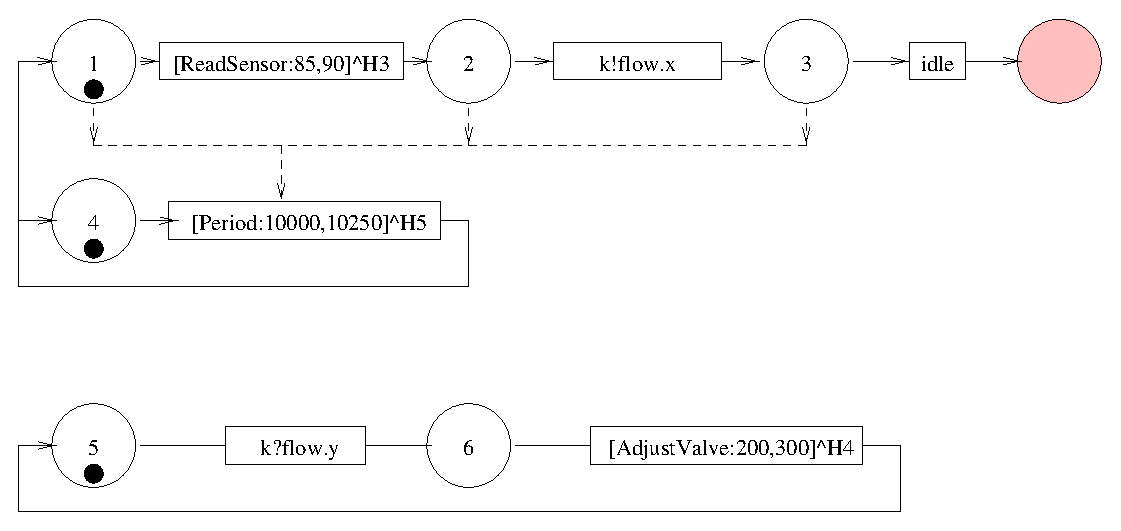
\includegraphics[width=.8\linewidth]{TGGEN/valvenet.eps}
\end{center}
\caption{Net for the flow regulator\label{fig:tgvalvenet}}
\end{figure}   

Finally, the TA is constructed by applying the algorithm of
Figure~\ref{fig:tgmkgraph}, starting from the initial location
$(\W,\NN,\D)$, where the initial marking $\W = \{1,4,5\}$; the initial
state of the network $\NN = \{\kk \mapsto (\free,\emq)\}$ i.e., the
condition of channel $\kk$ is \emph{free} and its pending message
queue is \emph{empty}; and the initial data environment $\D = \{x
\mapsto \undefined, y \mapsto \undefined\}$. 

The final TA has 48 locations, 146 edges, and uses 5 clock
variables. It is shown in full in Appendix~\ref{app:flowta}. Many of
the locations and edges in the generated TA are redundant, in the
sense that some locations are unreachable and some edges are guarded
by clock constraints which are unsatisfiable. This is typical of many
automatic translators~\cite{yov:93,bra:95,her:98}. Since the clock
constraints are not used to guide the construction of the TA, the
worst-case complexity of the translation is comparable to that for an
untimed language, i.e., exponential in the number of processes,
channels and data variables. A more careful analysis of the clock
constraints would allow many of the redundancies to be eliminated,
although the fundamental complexity of the problem remains the
same. This approach has not been implemented. Instead, it will be seen
that an alternative approach presented in Chapter~\ref{chap:sggen}
addresses the problem in a way which appears to be effective in
practice. Note also that it is possible to improve the quality of the
generated TA by using a clock optimisation tool such as
OptiKron~\cite{daw:98a}, which produces an equivalent TA having a
reduced number of clocks. For the example given here, OptiKron reduces
the number of clocks required from~5 to~4.

Once the TA has been generated, a model-checking tool, such as KRONOS,
can be used to ensure that the model exhibits desirable properties.
For example, the simple bounded response property that the $AdjustValve$
operation is always enabled within 300 time units of the enabling of the
$ReadSensor$ operation, can be expressed in TCTL as
\begin{zed}
init \implies \aalways{} (enable(ReadSensor) \implies 
              \aeventually{\leq 300} enable(AdjustValve))
\end{zed}
Let {\tt flow.tctl} be a file containing a statement of this property
in the syntax expected by KRONOS:
\begin{verbatim}
init IMPL AB (enable(OP_ReadSensor) IMPL 
             (AD{<=300} enable(OP_AdjustValve)))
\end{verbatim}
Let {\tt flow.tg} be a file containing the TA generated from the 
\bcandle\ model.
The property can be checked in a forward reachability analysis using the
command
\begin{verbatim} 
kronos -forw flow.tg flow.tctl
\end{verbatim}
giving the result
{
\scriptsize
\begin{verbatim} 
kronos: release 2.4.4 (i686) date Tue Aug 29 16:16:08 WET DST 2000
kronos: file flow.kro already exists 
kronos: reading file flow.kro...
kronos: begin evaluation of flow.tctl
kronos: begin forward analysis
kronos: 14 simulation states generated
kronos: 14 simulation transitions generated
kronos: Invariance *** TRUE ***
kronos: end evaluation of flow.tctl
kronos: compacting

---------------------------------------------------------------------------
kronos: fixpoint          : system   0.010s * user   3.410s * #iterations 17
kronos: compact time      : system   0.000s * user   0.000s *
kronos: forward analysis  : system   0.000s * user   0.010s *
kronos: total time        : system   0.010s * user   3.460s *
---------------------------------------------------------------------------
\end{verbatim}
} 

Another property can be stated and checked, concerning the
periodicity and jitter of the enabling of $AdjustValve$, for example,
\begin{zed}
init \implies \aeventually{} enable(AdjustValve) \land \\
\t1 \aalways{} (enable(AdjustValve) \implies \\ 
\t2              \aeventually{\leq 100} ((\aalways{<9885} \lnot enable(AdjustValve)) \land \\
\t3 \hspace*{2ex}\;(\aeventually{<=10165} enable(AdjustValve))))
\end{zed}
which states that $AdjustValve$ is eventually enabled and, whenever
enabled, it fires within 100 time units, remaining disabled thereafter
until it becomes enabled again after no less than 9885, and no more
than 10165, time units. KRONOS verifies this property also.

The stated bounds (9885 and 10165) are as tight as possible for this
example and, even for such a simple model, are not obvious by
inspection. An analysis of this sort helps to build confidence in the
quality of control which may be supplied by an implementation of the
flow regulator.

In fact, there is a hidden assumption in the interpretation, given
above, of the periodicity property: that whenever $AdjustValve$ is
enabled, it becomes disabled only by firing, and not as the result of
an interrupt or timeout. In this case, the correctness of the
assumption can be seen immediately by inspection of the
model. However, in general, this may not be straightforward and one
would like to be able to state the property in TCTL and check it using
KRONOS. As Hernalsteen has observed~\cite{her:98}, it is not so easy
in TCTL to state properties concerning the firing of transitions as
opposed to their enabling.  This is because TCTL is a state-based,
rather than an event-based, logic.  The firing of a transition can be
checked only by encoding this event somehow in the discrete state of
the model. If the encoding is done by the modeller in an ad-hoc
fashion, there is the possibility that errors will be introduced into
the model; if it is done automatically for all events by the
translator, the size of the state space will be increased, perhaps
unnecessarily. One possible solution is to allow some events to be
marked by the user for `tracking' in the model, so that the translator
can automatically add the encodings required only for those events of
interest. Alternatively, one could consider the use of a logic in
which both states and events can be referenced.

\section{Conclusions}\label{sec:tgconc}
In this chapter, we have presented a translation to timed automata of
the timed process language \bcandle. The translation closely follows
the semantic rules of the language and can be shown to be correct in a
straightforward manner. We have also described an efficient method by
which the translation can be implemented. The method adapts and
extends techniques which have proved effective in similar
settings~\cite{gar:92,yov:93}. A translator has been implemented and
has been applied to a number of examples. As a result of this work, it
is now possible, for the first time, to apply automatic analysis
techniques, such as model checking, to system models which are
described using a timed language which provides value-passing,
prioritised, broadcast communication over latent channels as a primitive
construct. 












